\documentclass[en]{../../../eplsummary}

\graphicspath{{img/}}

\hypertitle{Design of Embedded and real-time systems}{8}{INGI}{2315}
{Master students 2018--2019}
{Jean-Didier Legat}

\newpage

\section{Getting Started}

\begin{enumerate}
  
    \item \textbf{Give the main peripherals (or IOs) connected to: (a)  the FPGA portion of the DE10-Nano and (b) the HPS of the DE10-Nano}
   
    \begin{multicols}{2}
    For the HPS (Hard Processor System):
    \begin{itemize}
        \item LTC 2x7 Header (connector)
        \item USB 2.0 PHY 
        \item USB 2.0 OTG 
        \item DDR3 Memory
        \item UART to USB 
        \item G - sensor
        \item Gigabit Ethernet
        \item User Push Buttons
        \item Micro SD Card Socket 
    \end{itemize}
    
    For the FPGA: 
    \begin{itemize}
        \item Arduino Header
        \item 2x20 GPIO headers
        \item Slide Switch x4 
        \item User push button x2
        \item 2x5 ADC Header and analog input
        \item LED x8
        \item HDMI TX Interface
        \item[\vspace{\fill}]
        \item[\vspace{\fill}]
    \end{itemize}
    
    \end{multicols}
    
    \vspace{5pt} \hrule
    
    \item \textbf{How many USB interfaces the DE10-Nano has and what are their function?}
    
    There are 3 USB interfaces:
    \begin{itemize}
        \item mini USB blaster II to connect to the FPGA
        \item mini USB phy for the UART interface for communication with the HPS (host and device mode)
        \item micro USB for the OTG (to connect keyboard, mouse,\dots)
    \end{itemize}
    
    \vspace{5pt} \hrule
  
    \item \textbf{How many Systems LEDs the DE10-Nano has and what are they function?}
    
    There are 11 in total:  
    \begin{itemize}
        \item 8 for personal use of the user
        \item 1 as power light indicator 
        \item 2 as indicator for UART communication (Tx-Rx) % Je crois
        \item 2 as indicator for JTAG communication (Tx-Rx)
        \item 1 as CONF DONE when FPGA is successfully configured
        \item 1 as 3.3 V when the 3.3 V is available
    \end{itemize}
 
    \vspace{5pt} \hrule
  
    \item \textbf{Give the different stages of a typical boot flow.}
    
    There are 3 stage (simplified version): Reset, Boot ROM, Preloader.
    
   \begin{figure}[H]
       \centering
       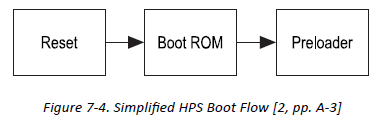
\includegraphics[scale = 1]{bootflow.PNG}
   \end{figure}
   
   The complete version is:
   
   \begin{figure}[H]
       \centering
       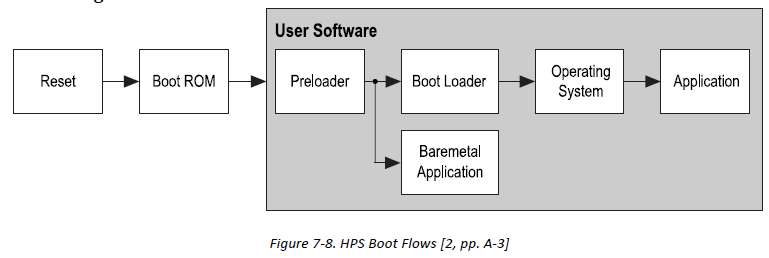
\includegraphics[scale = 0.85]{bootHP.PNG}
   \end{figure}
   
   Booting software on the HPS is a multi-stage process. Each stage is responsible for loading the next stage.
      
    \vspace{5pt} \hrule
  
    \item \textbf{Explain the functions of the BootROM stage.}
    
    The first software stage is the BootROM. The BootROM code locates and executes the 2nd software stage, called the Preloader. This code \textbf{can not be changed} and is used exclusively for booting the HPS.
    
    The BootROM offers the following features:
    \begin{itemize}
        \item 64 KB size
        \item Contains the code required to support HPS boot from cold or warm reset
    \end{itemize}

    \vspace{5pt} \hrule
  
    \item \textbf{Explain the functions of the Preloader.} 
    
    The Preloader is one of the most important boot stage. It is actually what one would call the boot “source”, as all stages before it are unmodifiable. The Preloader
    and subsequent software stages are collectively referred to as user software. The program locates, and IF PRESENT, executes the next software stage. The Preloader can be stored on external flash-based memory, or in the FPGA fabric.

%The SOFTWARE that configures the HPS I/O PINS is called the PRELOADER. \\ 

    The Preloader typically performs the following actions: 
    \begin{itemize}
        \item Initialize the SDRAM interface
        \item Configure the IOs of the HPS through the "scan manager"
        \item Configure the pin multiplexing through the "system manager"
        \item Configure the HPS clock through the "clock manager"
        \item Initialize the flash controllers that contain the next stages of the boot program
        \item Load the boot program in the SDRAM and give it control
    \end{itemize}
    
    \vspace{5pt} \hrule
  
    \item \textbf{Explain the functions of the Bootloader.}
    
    There are 3 stages before a Linux application can be launched:
    \begin{itemize}
        \item Preloader
        \item Bootloader
        \item Operating System
    \end{itemize}
    
    The second step is to obtain a Bootloader that is capable of loading the Linux kernel.
    
    The Bootloader finds and loads the firmware which is supposed to run on the chip.
 
    \vspace{5pt} \hrule
  
    \item \textbf{Explain how the Hardware-to-Software Handoff is implemented.}
    \begin{itemize}
        \item FPGA-to-HPS bridge: a high performance bus with a configurable data width of 32, 64, or 128 bits.
        \item HPS-to-FPGA bridge: a high performance bus with a configurable data width of 32, 64, or 128 bits.
        \item Lightweight HPS-to-FPGA bridge: a bus with a 32-bit fixed data width.
        \item FPGA manager interface: signals that communicate with the FPGA fabric for boot and configuration.
        \item Interrupts: allows soft IPs to supply interrupts directly to the MPU interrupt controller.
        \item HPS debug interface: an interface that allows the HPS debug control domain to extend into the FPGA.
    \end{itemize}
    
    \vspace{5pt} \hrule
    
    \item \textbf{Give the different ways the FPGA can be configured.}
    
    \begin{itemize}
        \item Via JTAG (Quartus Prime Programmer)
        \item Via Bootloader in the SD (via \texttt{SOC\_system.rbf})
    \end{itemize}

    Configuration of the FPGA portion of the device starts when the FPGA portion is released from reset state (for example, on power up). The control block (CB) in the FPGA portion of the device is responsible for obtaining an FPGA configuration image and configuring the FPGA. The FPGA configuration ends when the configuration image has been fully loaded and the FPGA enters user mode. The FPGA configuration image is provided by users and is typically stored in non-volatile flash-based memory. The FPGA CB can obtain a configuration image from the HPS through the FPGA manager, or from another external source, such as the Quartus Prime Programmer.
    
    \vspace{5pt} \hrule
  
    \item \textbf{Describe the different boot options of the Cyclone V SoC.}
    
    The processor can boot from the following sources:
    \begin{itemize}
     \item NAND flash memory through the NAND flash controller
     \item SD/MMC flash memory through the SD/MMC flash controller
     \item SPI and QSPI flash memory through the QSPI flash controller using Slave Select 0
     \item FPGA fabric on-chip memory
    \end{itemize}
     
    The choice of the boot source is done by modifying the BOOTSEL and CLKSEL values \textbf{before the device is powered up}. Therefore, the Cyclone V device normally uses a \textbf{physical dip switch} to configure the BOOTSEL and CLKSEL.
    
    The DE0-Nano-SoC can \textbf{only boot} from \textbf{SD/MMC} flash memory, as its BOOTSEL and CLKSEL values are hard-wired on the board. Although its HPS contains all necessary controllers, the board doesn’t have a physical DIP switch to modify the BOOTSEL and CLKSEL values
 
    \vspace{5pt} \hrule
  
    \item \textbf{Describe in detail the three HPS-FPGA Interface Bridges.}
    
    The HPS-FPGA interfaces include:
    \begin{itemize}
        \item \textbf{FPGA-to-HPS bridge}: a high performance bus with a configurable data width of 32, 64, or 128 bits. It allows the FPGA fabric to master transactions to slaves in the HPS. This interface allows the FPGA fabric to have full visibility into the HPS address space.
        
        \item \textbf{HPS-to-FPGA bridge}: a high performance bus with a configurable data width of 32, 64, or 128 bits. It allows the HPS to master transactions to slaves in the FPGA fabric. It is sometimes called the “heavyweight” HPS-to-FPGA bridge to distinguish its “lightweight” counterpart (see below).
        
        \item \textbf{Lightweight HPS-to-FPGA bridge}: a bus with a 32-bit fixed data width. It allows the HPS to master transactions to slaves in the FPGA fabric.
        
    %    \item \textbf{FPGA manager interface} – signals that communicate with the FPGA fabric for boot and configuration.
        
    %    \item \textbf{Interrupts} – allows soft IPs to supply interrupts directly to the MPU interrupt controller.
        
    %    \item \textbf{HPS debug interface} – an interface that allows the HPS debug control domain to extend into the FPGA.
    \end{itemize}
 
    \vspace{5pt} \hrule
  
    \item \textbf{Explain how the peripherals implemented in the FPGA logic can be accessed and describe the other interfaces between the FPGA and the HPS.}
    
    Accessing the FPGA peripherals connected to the HPS’ lightweight HPS-to-FPGA bridge is quite simple, as no libraries are needed. One can simply use the low-level functions listed below to address the peripherals at an offset from the lightweight HPS-to-FPGA bridge’s base address.
    \begin{itemize}
    \item \texttt{alt\_write\_byte(dest\_addr, byte\_data)}
    \item \texttt{alt\_read\_byte(src\_addr)}
    \item \texttt{alt\_setbits\_byte(dest\_addr, byte\_data)}
    \item \texttt{alt\_clrbits\_byte(dest\_addr, byte\_data)}
    \item \texttt{alt\_xorbits\_byte(dest\_addr, byte\_data)}
    \item \texttt{alt\_replbits\_byte(dest\_addr, msk, byte\_data)}
    \end{itemize}

    \vspace{5pt} \hrule
    
    \item \textbf{Explain the difference between a Linux environment and a Bare-Metal one.}

    \textbf{Bare-metal Application}
    
    A bare-metal software has no OS overhead.
    
    \begin{itemize}
    \item Advantages
    \end{itemize}
    
    Code executes at native speed as no context switching is ever performed.
    
    Code can directly address the HPS peripherals using their \textbf{physical} memory-mapped addresses, as no virtual memory system is being used.
    
    \begin{itemize}
    \item Disadvantages
    \end{itemize}
    
    The programmer must continue to configure the Cyclone V to use all its resources (e.g. to release CPU1 from reset).
    Supposing CPU1 is available for use, it is still difficult to run multi-threaded code, as an OS generally handles program scheduling and CPU affinity for the programmer.
    
    \textbf{Application Over an Operating System (Linux)}
    
    The code is run over a Linux operating system.
    
    \begin{itemize}
    \item Advantages
    \end{itemize}
    
    The kernel releases CPU1 from reset upon boot, so all processors are available
    This is possible since the Linux kernel has access to a huge amount of device drivers.
    Multi-threaded code is much easier to write, as the programmer has access to the familiar OS facilities for threading.
    The Linux kernel is not restricted to running compiled C programs as long as you first install the runtime environment required.
    
    \begin{itemize}
    \item Disadvantages
    \end{itemize}
    
    A program cannot directly access the HPS peripherals through their physical memory-mapped addresses. Instead, one first needs to map the physical addresses of interest into the running program’s virtual address space.
    Ideally, the programmer should write a device driver for each specific component that is designed in order to have a clean interface between user code and device accesses.

    \vspace{5pt} \hrule
    
    \item \textbf{Describe the different ways to access the DE10-Nano board at run time and for development.}
    
\end{enumerate}

\newpage

\section{Discovering the Cyclone V SoC}

\begin{enumerate}
    \item \textbf{Explain the main features of a LAB and MLAB.}
    
    LABs (Logic Array Blocks) are configurable logic bocks. They contain the necessary logic to conduct the signal to their ALM (Adaptive Logic Module).
    
    MLABs (Memory LABs) contain the LABs. They are either used for logic blocks or as small memories. 
  
    \vspace{5pt} \hrule
  
    \item \textbf{Explain the main features of a ALM and its different operating modes.}
    
    Each ALM contains 4 registers. Each one of these registers has 4 distinct ports:
    \begin{itemize}
        \item Data
        \item Clock
        \item Synchronous and asynchronous clear
        \item Synchronous load
    \end{itemize}
    
    The Cyclone V ALMs have 4 different modes:
    
    \begin{enumerate}
        \item \textbf{Normal mode}: This mode allows 2 functions to be implemented in 1 ALM, or a single function of more than 6 inputs. Up to 8 inputs coming from the local interconnexion of the LAB can be inputs in the combinatory logic.
        
        \item \textbf{Extended LUT mode}: In this mode, if the 7-inputs function is not registered, then the non-used $8^{th}$ input, is available for "register packing".
        
        \item \textbf{Arithmetic mode}: This mode uses 2 sets of 4-input LUT, as well as 2 full-adders.
        
        \item \textbf{Shared Arithmetic mode}: Can implement a 3-input adder within the ALM. This mode configures the ALM with 4 4-input LUT. Each of these LUTs computes the sum of 3 inputs or the "carry" of these 3 inputs. The output of the carry computation feeds the next adder by using a connection called "shared arithmetic chain".
        
    \end{enumerate}
    
    \vspace{5pt} \hrule
  
    \item \textbf{Describe the types of embedded memory that the Cyclone V contains. For each of them, give an approximate capacity (in Kb) for the Cyclone V in the DE10-Nano kit.}
    
    The Cyclone V devices contain two types of memory blocks:
    
    \begin{enumerate}
        \item 10 Kb M10K blocks: blocks of dedicated memory resources. The M10K blocks are ideal for larger memory arrays while still providing a large number of independent ports. 
        
        Total capacity of those blocks for the Cyclone V: 5500 Kb.

        \item 640 bit memory logic array blocks (MLABs): enhanced memory blocks that are configured from dualpurpose logic array blocks (LABs). The MLABs are ideal for wide and shallow memory arrays. The MLABs are optimized for implementation of shift registers for digital signal processing (DSP) applications, wide shallow FIFO buffers, and filter delay lines. Each MLAB is made up of ten adaptive logic modules (ALMs). In the Cyclone V devices, you can configured these ALMs as then 32 x 2 blocks, giving you one 32 x 20 simple dual-port SRAM block per MLAB. 
        
        Total capacity of those blocks for the Cyclone V: 621 Kb.
    \end{enumerate}
    
    \vspace{5pt} \hrule
  
    \item \textbf{Give the general variable precision DSP blocks architecture (only the main resources). Explain how can be implemented an independent complex multiplication. How many DSP blocks does the Cyclone V in the DE10-Nano kit contain?}
    
    The following variable precision DSP block signals control the output register per variable precision DSP
    block:
    \begin{itemize}
        \item \texttt{clk[2..0]}
        \item \texttt{ena[2..0]}
        \item \texttt{aclr[1]}
    \end{itemize}
    
    For an independent complex multiplication: $$ (a+bj) \times (c+dj) $$

    The imaginary part $[(a \times d) + (b \times c)]$ is implemented in the first variable-precision DSP block, while the
    real part $[(a \times c) - (b \times d)]$ is implemented in the second variable-precision DSP block.
    
    \vspace{5pt} \hrule
  
    \item \textbf{Explain the main function of the SCU and ACP blocks?}
    
    Snoop control unit (SCU) ensures coherency between processors.
    
    Accelerator coherency port (ACP) accepts coherency memory access requests 
    
    \vspace{5pt} \hrule
  
    \item \textbf{How many caches does the HPS have and what are their capacity?}
    
    Cache memory that is closely coupled with an associated processor is called level 1, or L1 cache. Each
    Cortex-A9 processor has two independent 32 KB L1 caches (one for instructions and one for data)
    allowing simultaneous instruction fetches and data access. Each L1 cache is four-way set associative, with
    32 bytes per line, and supports parity checking.

    \begin{itemize}
        \item 32 KB instruction cache
        \item 32 KB data cache 
        \item 512 KB L2 shared cache
    \end{itemize}

    \vspace{5pt} \hrule
  
    \item \textbf{Explain the main features of these serial interfaces: I2C, UART, CAN, SPI.}
    
    \begin{itemize}
    
    \item The I2C controller provides support for a communication link between integrated circuits on a board. It is a simple two-wire bus which consists of a serial data line (SDA) and a serial clock (SCL) for use in applications such as temperature sensors and voltage level translators to EEPROMs, A/D and D/A converters, CODECs, and many types of microprocessors. 

    The four I2C controllers are based on Synopsys DesignWare APB I2C controller which offer the following features:
    \begin{itemize}
        \item Two controllers support I2C management interfaces for use by the EMAC controllers
        \item Support both 100 KBps and 400 KBps modes
        \item Support both 7-bit and 10-bit addressing modes
        \item Support master and slave operating mode
        \item Direct access for host processor
        \item DMA controller may be used for large transfers
    \end{itemize}

    \item The UART controllers are based on an industry standard 16550 UART controller. The UART controllers are instances of the Synopsys DesignWare APB Universal Asynchronous Receiver/Transmitter (DW-apb-uart) peripheral. 
    The HPS provides two UART controllers to provide asynchronous serial communications. The two UART modules are based on Synopsis DesignWare APB Universal Asynchronous Receiver/ Transmitter peripheral and offer the following features:
    \begin{itemize}
        \item 16550-compatible UART
        \item Support automatic flow control as specified in 16750 standard
        \item Programmable baud rate up to 6.25 MBaud (with 100MHz reference clock)
        \item Direct access for host processor
        \item DMA controller may be used for large transfers
        \item 128-byte transmit and receive FIFO buffers 
    \end{itemize}

    \item The two CAN controllers are based on the Bosch D\_CAN controller and offer the following features:
    
    \begin{itemize}
        \item Compliant with CAN protocol specification 2.0 part A \& B
        \item Programmable communication rate up to 1 Mbps
        \item Holds up to 128 messages
        \item Supports 11-bit standard and 29-bit extended identifiers
        \item Programmable interrupt scheme
        \item Direct access for host processor
        \item DMA controller may be used for large transfers 
    \end{itemize}
    
    \item The two SPI (serial peripheral interface) master controllers are based on Synopsis DesignWare Synchronous Serial Interface (SSI) controller and offer the following features:
    
    \begin{itemize}
    \item Choice of Motorola* SPI, Texas Instruments* Synchronous Serial Protocol or National Semiconductor*
    Microwire protocol
    \item Programmable data frame size from 4 bits to 16 bits
    \item Supports full- and half-duplex modes
    \item Supports up to four chip selects
    \item Direct access for host processor
    \item DMA controller may be used for large transfers
    \item Programmable master serial bit rate
    \item Support for rxd sample delay
    \item Transmit and receive FIFO buffers are 256 words deep
    \end{itemize}
    
    \item The two SPI slave controllers are based on Synopsys DesignWare Synchronous Serial Interface (SSI) controller and offer the following features:
    \begin{itemize}
        \item Programmable data frame size from 4 bits to 16 bits
        \item Supports full- and half-duplex moces
        \item Direct access for host processor
        \item DMA controller may be used for large transfers
        \item Transmit and receive FIFO buffers are 256 words deep
    \end{itemize}
    
    \end{itemize}

    \vspace{5pt} \hrule
  
    \item \textbf{Explain briefly the main features of the FPGA Manager.}
    
    The FPGA manager in the hard processor system (HPS) manages and monitors the FPGA portion of the system on a chip (SoC) device. The FPGA manager can configure the FPGA fabric from the HPS, monitor the state of the FPGA, and drive or sample signals to or from the FPGA fabric. 

    \vspace{5pt} \hrule
  
    \item \textbf{Give and explain the HPS-FPGA bridges block diagram and system integration.}
    
    \begin{figure}[H]
        \centering
        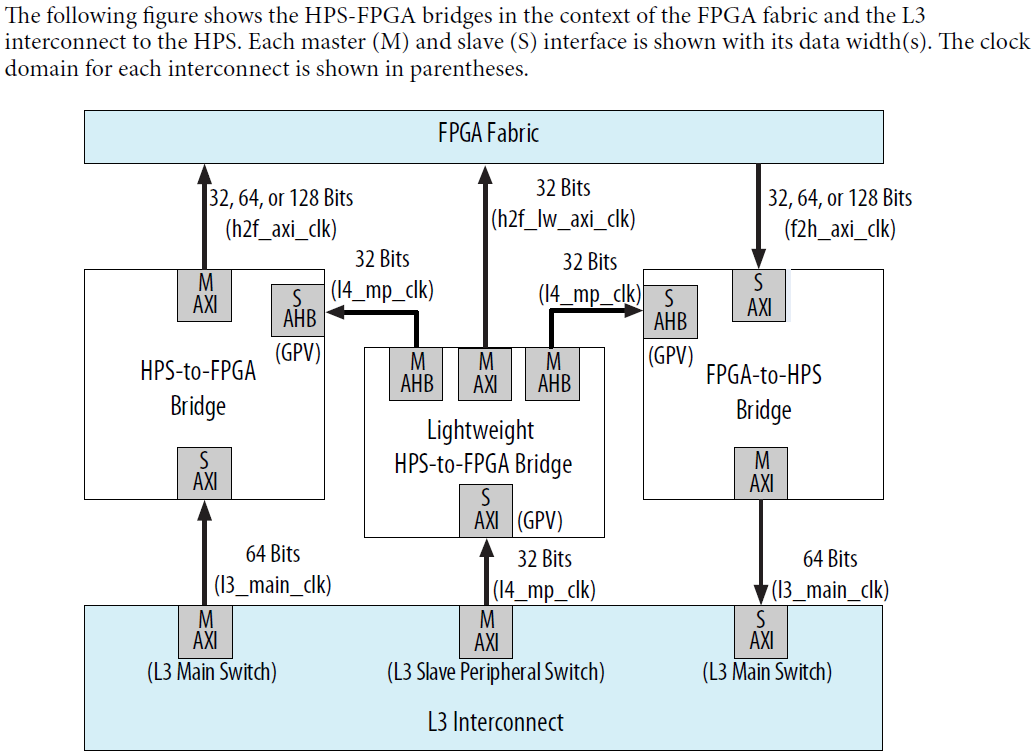
\includegraphics[scale =0.8]{bridge1.PNG}
    \end{figure}
    
    \begin{figure}[H]
        \centering
        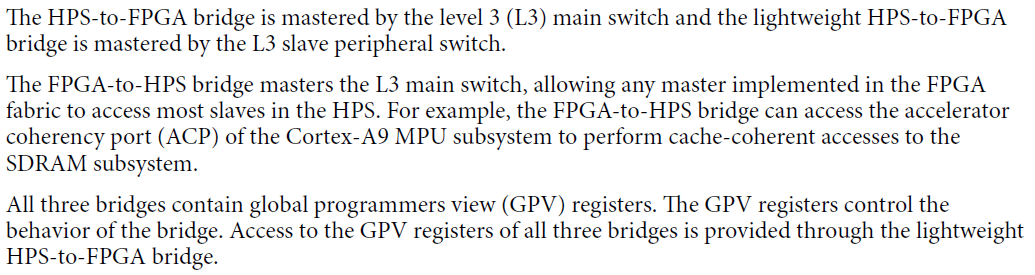
\includegraphics[width=0.7\textwidth]{bridge2.PNG}
    \end{figure}
    
    \vspace{5pt} \hrule
    
    \item \textbf{Sketch the block diagram of the ARM Cortex A9 MPCore and explain the principle of the NEON Media processing engine. }
    
    \begin{figure}[H]
        \centering
        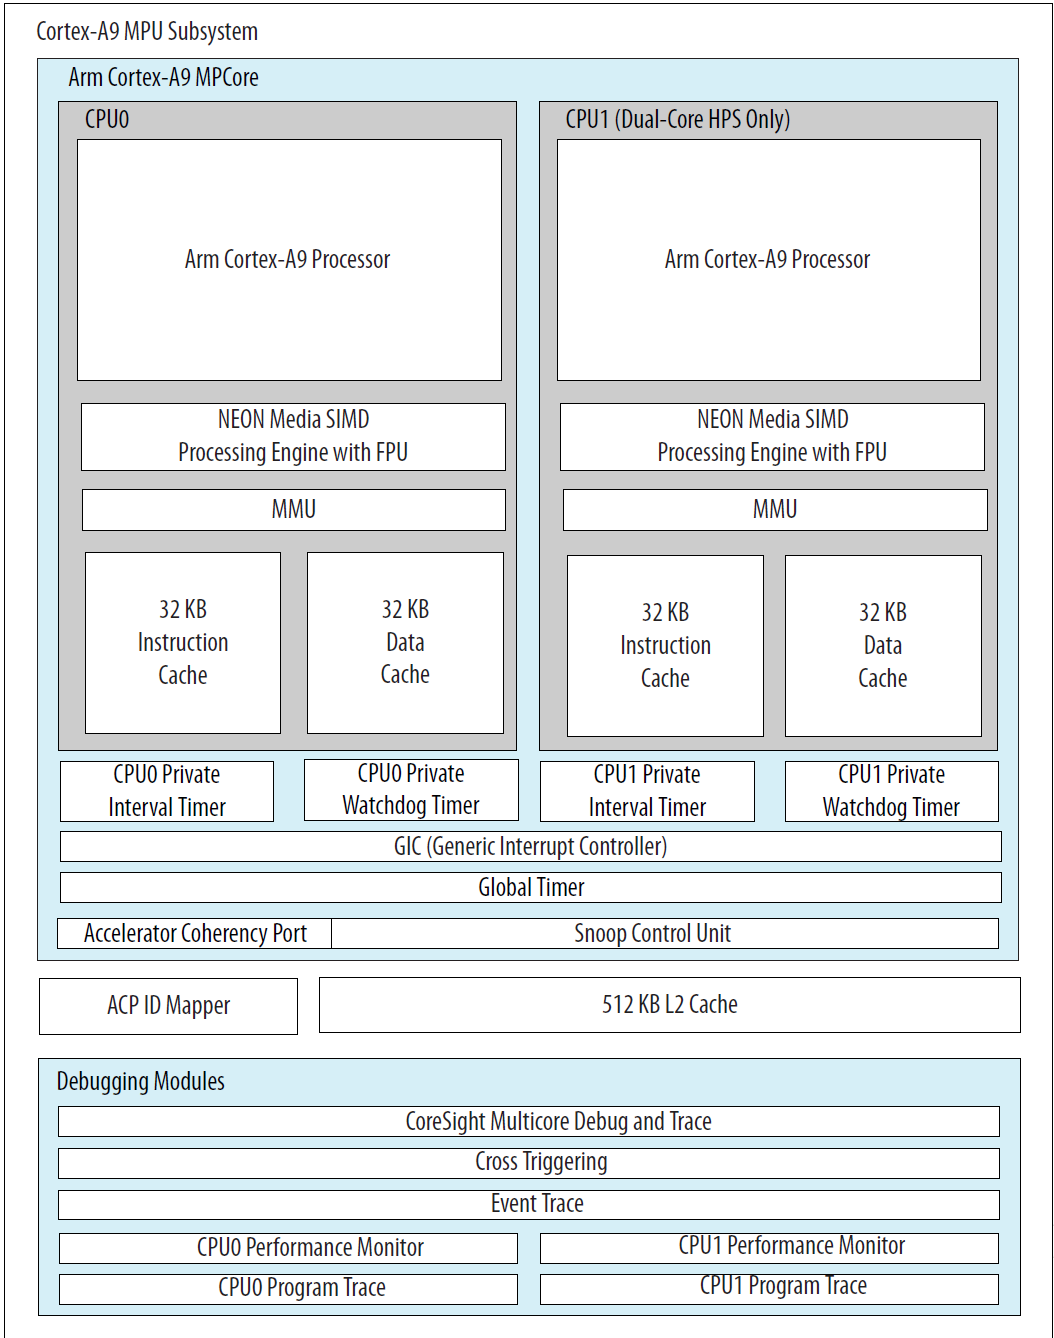
\includegraphics[scale =0.7]{arm1.PNG}
    \end{figure}
    
    \begin{figure}[H]
        \centering
        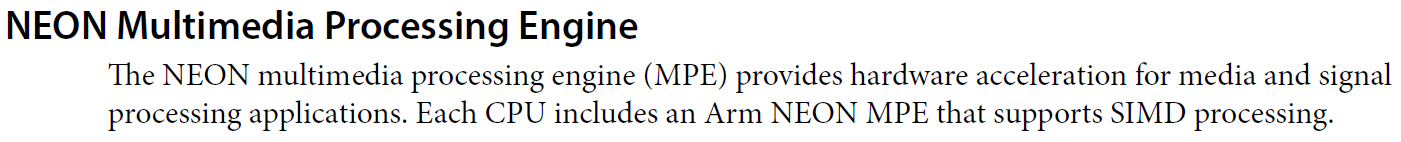
\includegraphics[scale =0.6]{arm2.PNG}
    \end{figure}

    \vspace{5pt} \hrule
  
    \item \textbf{Explain the concept of GHRD (Golden Hardware Reference Design).}
     

    The Golden Hardware Reference Design is an Intel Quartus Prime project that contains
    a full HPS design for the Cyclone V SoC / Arria V SoC Development Kit. The GHRD has
    connections to a boot source, SDRAM memory and other peripherals on the
    development board.
    
    For every new released version of SoC EDS, the GHRD is included in the SoC EDS
    tools. The GHRD is regression tested with every major release of the Intel Quartus
    Prime Design Software and includes the latest bug fixes for known hardware issues.
    The GHRD serves as a known good configuration of an SoC FPGA hardware system. 
    
    \vspace{5pt} \hrule
  
    \item \textbf{Explain the concepts of SMP and AMP modes.}
    Symmetrical vs. Asymmetrical Multiprocessing (SMP vs AMP)
    
    In SMP mode, a single OS instance controls both cores. The SMP configuration is
    supported by a wide variety of operating system manufacturers and is the most
    common and straightforward configuration mode for multiprocessing. 
    
    In the AMP (Asymmetrical Multi-Processing) configuration, two different operating
    systems or two instances of a single operating system run on the two cores. The two
    operating systems have no inherent knowledge of how they share CPU resources. To
    ensure efficient use of MPU subsystem resources in this environment, you must deal
    with several complex issues when designing your system.

    \vspace{5pt} \hrule
  
    \item \textbf{Explain the concept of Device Tree.}
    
    The Linux Device Tree is a data structure that describes the underlying hardware to the Linux operating system kernel. By passing this data structure the OS kernel, a single OS binary may be able to support many variations of hardware. This flexibility is particularly important when the hardware includes an FPGA. 
\end{enumerate}

\newpage

\section{Chapter 1: \textit{Real-time operating systems - things you really ought to know}}

\begin{enumerate}
    \item \textbf{Explain why time and timing data are important in embedded systems.}

    A large number of application needs the cooperation of continuous electronic systems and microprocessor-based systems. However, a big difference separates them. One is continuous and the other is discrete. 

    In continuous (“analog”) electronic systems all operations can, if required, take place simultaneously (“concurrently”). Not only that, but processing is done instantaneously. But this just isn't possible in processor-based systems as these are fundamentally discrete in operation.

    Moreover, the processing is done instantaneously which isn't just possible in processor-based system because of 2 big factors :
    \begin{itemize}
        \item Processor can do only one thing at a time
        \item Operations take time
    \end{itemize}
    
    And that's why it's important to begin development knowing your system timing needs.
    
    Timing is important in embedded systems and we have to keep in mind these design implications : 
    \begin{itemize}
        \item Tasks are intended to run to a completion point each time they are activated (so take a time Te)
        \item A practical system must have some spare time (Ts)
        \item Just because a code can run in a period doesn't mean its performance is acceptable
        \item Input-to-output processing delay ("latency") may cause problems with the behaviour of the overall system
    \end{itemize}
    
    \vspace{5pt} \hrule
    
    \item \textbf{Define the meaning of process and task.}
    
    A software process is also known as a task in the embedded world.
    \begin{itemize}
        \item A task represents the execution of a single sequential program
        \item A software process is defined by a combination  of code, data and processor
    \end{itemize}
    
    \vspace{5pt} \hrule
    
    \item \textbf{Explain the difference between periodic and aperiodic tasks.}
    \begin{itemize}
        \item Periodic : To be serviced at regular intervals. (Control loop)
        \item Aperiodic : To be serviced at random (and not preset) times
    \end{itemize}
    
    
    \vspace{5pt} \hrule
    
    \item \textbf{Explain what concurrency, quasi-concurrency and multitasking are.}
    \begin{itemize}
        \item Concurrency : is a property of systems in which several computations are executing simultaneously, and potentially interacting with each other. \textbf{(NOT FROM THE BOOK)}
        \item Quasi-concurrency : apparent concurrent execution of a set of individual processes (tasks). In other words, by using interrupts, we can run multiple tasks "simultaneously": a form of simple or "poor man's" multitasking.
        \item Multitasking : Run a number of tasks within a processor system. Single processor multitask designs are called "multitasking" systems. %not so sure about this one
    \end{itemize}
    
    \vspace{5pt} \hrule
    
    \item \textbf{Explain why interrupt-driven designs can be considered as a simple form of multitasking.}
    
    When using hardware interrupt \footnote{A signal that is applied electronically to the processor. When the interrupt is generated it invokes a predetermined response (as defined by the programmer) to execute some specified code.} each code unit runs and it has complete use of the computer resources; it appears to 'own' the processor. This means that we can design the software as if each function will run on its own processor, the 'abstract' processor. So what we have is the apparent concurrent execution of a set of individual processes (tasks), so-called 'quasi-concurrency'. In other words, by using interrupts, we can run multiple tasks 'simultaneously': a form of simple or 'poor man's' multitasking. 
    
    \vspace{5pt} \hrule
    
    \item \textbf{Give the basic features of RTOSs.}
    \begin{itemize}
        \item Task structuring of programs.
        \item Task implementations as logically separate units (task abstraction).
        \item Parallelism (concurrency) of operations.
        \item Use of system resources at predetermined times.
        \item Use of system resources at random times.
        \item Task implementation with minimal hardware knowledge.
    \end{itemize}
    
    
    
    \vspace{5pt} \hrule
    
    \item \textbf{Give the fundamentals of multi-tasking design.}
    
    In a multitasking system it is possible to have tasks that perform independent and separate functions, i.e. are functionally independent AND separate but interdependent tasks. This raises a number of interesting problems, the solutions being provided by the multitasking software of the operating system, see Figure \ref{multi}.
    
    \begin{itemize}
        \item Task scheduling : to decide WHEN and WHY tasks should run.
        \item Mutual exclusion : to police the use of resources shared between tasks, to prevent damage or corruption to such resources
        \item Synchronization and data transfer : tasks must be able to 'speak' to each other, communication facilities are needed
    \end{itemize}
    
    \begin{figure}[H]
        \centering
        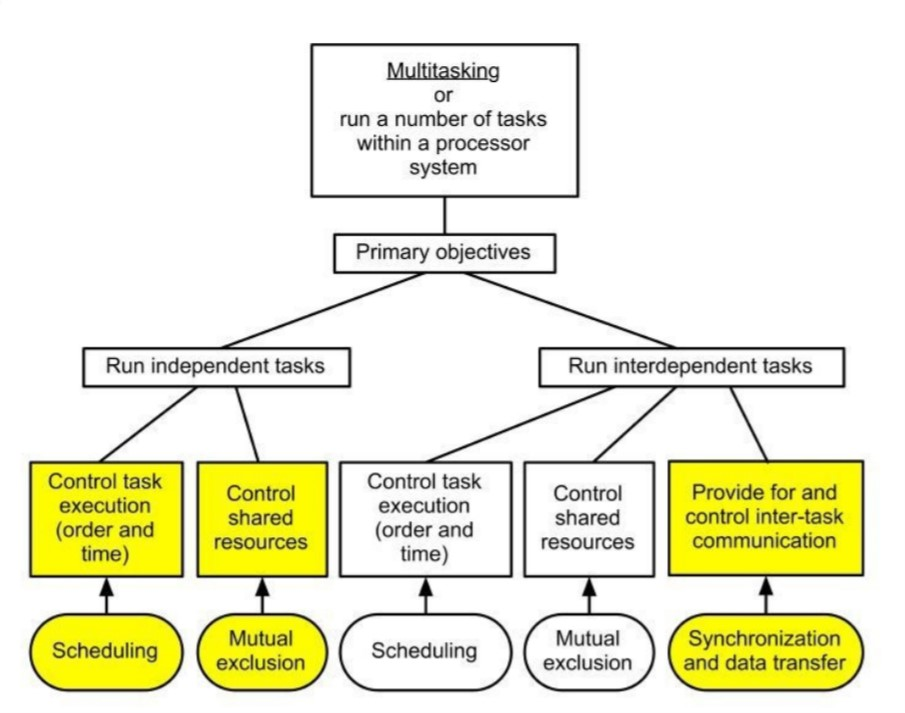
\includegraphics[scale =0.6]{Multitasking.jpg}
        \caption{}
        \label{multi}
    \end{figure}
    
\end{enumerate}

\newpage

\section{Chapter 2: \textit{Concepts and implementation}}

\begin{enumerate}
    \item \textbf{Explain the basis of simple cyclic, timed cyclic, round-robin and priority preemptive scheduling algorithms. Appreciate the merits and drawbacks of the various techniques.}
    
    \begin{itemize}
        \item Simple cyclic : first-in-first-out (FIFO) scheduling. The CPU is like a truck and the tasks or processes are like the drivers. The drivers form a queue, the 'head of the queue'  is given the full use of the truck until his work is done and the truck is given to the second driver.
        \begin{itemize}
            \item Aren't critical to the operation of the 
            system.
            \item Aren't time critical and 
            \item Run to completion each time they're executed.
        \end{itemize}
        Utilization: U = 100 \%.
        \item Timed cyclic: 
        \begin{itemize}
            \item Tasks are run repeatedly when the system is operational and 
            \item run to completion each time they're executed.
            \item Must be re-run at predetermined time intervals.
        \end{itemize} 
         Utilization: U = (Cycle time - Idle time)/Cycle time.
        The execution of the task set can be done at predefined intervals, the 'cyclic time'.
        \item Round-robin (time slicing): Tasks are still carried out on FIFO basis but now each driver has a fixed time for the use of the truck, the 'time slice'. When time is up, the current task is stopped and it will be resumed in the next allocated time slot.
        Its advantages are improved responsiveness and better use of shared resources. But in practice, it needs to be modified because tasks:  
        \begin{itemize}
            \item Vary in importance
            \item Don't always run at regular intervals
            \item May only run when specified conditions are met.
        \end{itemize} 
        \item Priority preemptive scheduling algorithms: In reality a particular execution order may be required, and so tasks are allocated priorities. The order can either be fixed (static priority scheme) or it can be changed during the program execution (dynamic priority scheme). Dynamic priority schemes improve flexibility and responsiveness. 
    \end{itemize}
    \vspace{5pt} \hrule
    \item \textbf{Explain the reason for using ready and suspended queues.}
    
    In reality tasks are not always ready, they may have to wait until specific conditions are met before becoming runable. Those tasks are said to be in the blocked or suspended state and are held in the waiting or suspended queue.
    

    \vspace{5pt} \hrule
    \item \textbf{Explain how queue ordering is changed at reschedule time in both priority and non-priority scheduling schemes.}
    


    \vspace{5pt} \hrule
    \item \textbf{Give the roles of the task control block (TCB) and the process descriptor.}
    
    Information held in the TCB enables the executive to control all scheduling activities.
    
    Task control block structure:
    \begin{itemize}
        \item Identifies the task
        \item Shows whether the task is ready to run or is suspended
        \item Defines the priority of the task within the system
        \item Gives the identifier of the task which follows. This is applied for the ready queues, suspended queues, and any other queues which may be used in the system. This field is used only when tasks queues are organized using linked list construct.
    \end{itemize}
    
    Process Descriptor: Dynamic information concerning the state of the process (task) that is held in the process descriptor. Each task has its own private PD and, in some designs, the descriptor may be located in the TCB itself.
    
    The TCB and Process Descriptor both contain dynamic information. Thus they have to be located in the read/write memory, usually RAM.

    \vspace{5pt} \hrule
    \item \textbf{Explain the concept of priorities and system responsiveness.}
    
    High priority tasks of the 'fast service queue' type are readied only when service is required, using interrupt signalling. When task execution is tied with the tick, some time variation or 'jitter' is experienced. This is small for the higher-priority jobs, getting larger as priorities reduce. Only tasks that can tolerate quite slow responses are implemented at the lowest level.
    
    The tick period has a significant influence on the system responsiveness. If a task having a higher priority than the running one, task pre-emption takes place. The running task is returned to the head-of- queue-position and its place is taken by the newest task. To support this strategy each task is given a specific priority.

    \vspace{5pt} \hrule
    \item \textbf{Explain why special interrupt handling routines may by-pass the scheduler in critical situations.}
    
    In most circumstance the scheduler handles all tasking operations. For instance, when an interrupt occurs, the interrupt handler readies the appropriate task; it doesn't dispatch it - that is the responsibility of the scheduler. The task joins the ready queue at a position determined by its priority, which could result ion a long delay between the interrupt requesting service and actually getting it. To cope with such issues, we can employ special interrupt service routines that completely by-pass the operating system. They have higher priority than that of the tick. What the ISRs do depends on system applications, design requirements and the exceptions that invoked them in the first place.


    \vspace{5pt} \hrule
    \item \textbf{Explain why code re-entrancy is essential in multitasking systems.}
    
    The most widely-used building blocks of modern programs are the subprogram and subroutine. In a multitasking system, each application process (task) is written separately and the object code loaded  into separate sections of memory. As a result tasks may appear to be independent, but this isn't true. They are interlinked via their commmon program building blocks, the subprograms or subroutines. Each task is allocated its own private stack and workspace. All subprogram parameters are normally kept on the stack, all local variables residing in the workspace. Now shared code can be used with safety because each task keeps its own data to itself. Such code is said to be 're-entrant'.


    \vspace{5pt} \hrule
\end{enumerate}

\newpage
%Coucou alexandre! :) 
%Coucou alexandre! :) 
%Coucou alexandre! :) Hello ! Tu étudies dure je vois ;) On travaille lentement mais surement :p 
% tout ce que tu vois autour de toi, c'est nous! ;P 
%(en toute humilité bien sur) EVidemment ! :D En tout cas un tout grand merci pour tout ça c'est vachement sympa de votre part d'avoir aussi bien avancé l'a dessus 
% C'est avec grand plaisir ;) Et puis si on peut contribuer à la réussite d'un max de gens, c'est qd mm trop cool ;) L'esprit d'entre-aide il n'y a que ça de vrai ;)   
\section{Chapter 3: \textit{Control of shared resources - mutual exclusion}}

\begin{enumerate}
    \item \textbf{Explain what mutual exclusion is and what it does.}
    
    Mutual exclusion is a property of concurrency control. It allows to deal with contention problems. It means that we use mutual exclusion strategy to tackle any problems if 2 tasks need the same hardware or store area.
    Example : the single flag method.
    
     \vspace{5pt} \hrule
    
    \item \textbf{Explain the difference between busy-wait and suspend-wait mutual exclusion methods. Give the advantages of the suspend-wait technique.}
    
    The single flag technique is simple to implement, easy to use with proper design and safe. Unfortunately it isn't very efficient. When a task finds the flag set, it goes into an open loop. It remains in a 'busy-wait' mode for the duration of the time slice. It results in wasted processor time and reduces the processor performance. 
    
    The task needs to give up the processor when it finds its way blocked. That is, it should suspend, thus allowing another task to instantly use the processor. Such an approach is called 'suspended-wait' and can be implemented in a number of ways. (p.48)
    
    Technique: Employ constructs specifically designed to support suspended-wait operations: semaphore, mutex and monitor.
    
    \vspace{5pt} \hrule
    
    \item \textbf{Explain why certain operations must be atomic.} 
    
    We said of an operation that it is atomic when we can't separate it. Instructions such as checking and setting the status of the flag must be an atomic operation. If it isn't the case, a user 1 could be pre-empted after loading up the variable but before changing its status. 
    
     \vspace{5pt} \hrule
     \item \textbf{Explain the concept and use of the binary and counting semaphores. Show how the mutex improves on the semaphore.}
     
    \textbf{Binary semaphore :} It can be seen as the software equivalent to an access control mechanism of a one-place parking. Initially the resource is free, the first operation is to provide the attendant with this status information. This corresponds to the initialization of the semaphore. When a user wants to use the resource, he approaches the barrier and presses the request button. In semaphore this is defined to be a "wait on semaphore" operation. If the resource is free, then the barrier is raised, user passes and the barrier is lowered. If then another user arrives, he gets a \textit{Wait} response and is redirected in the waiting queue (this corresponds to a task suspension). When the user leaves the parking, it generates a \textit{Signal}, the attendant status is updated and a "pass"-message is sent to the waiting queue. To manage the waiting queue there exist 2 basic methods: the FIFO (first-in-first-out) and the priority pre-emption method.
    
    \textbf{Counting semaphore :} Suppose the single resource is restructured so that it consists of a number of identical items. For instance it could be a set of local area network queues, used to store messages for onward transmission. Given this arrangement it is safe to let more than one task access the resource provided they don't use the same queue.
    
    Semaphore construct consists of a range of values, initially put on the maximum value (e.g. 4 queues). Each value corresponds to a specific instance of the resource (one queue). When a user wants to access the store, he first checks the resource (a queue) is available (semaphore value $\neq$ 0) and in that case it decrements the semaphore value by 1. When a user has finished it increments the semaphore value by one.
    
    The \textbf{mutex} is very similar to a semaphore but is specifically intended to control access to shared resources i.e. MUTual EXclusion (remember, the semaphore is essentially a flow control mechanism). It could be \textit{lock} (Wait) or \textit{Unlock} (Signal).
    A mutex differs diffes from a semaphore in one critical way: the task that release the mutex (Unlock) is the one that locked it in the first place. Thus we can consider the locking task to own the mutex. (p.55).
    

    \vspace{5pt} \hrule
    
    \item \textbf{Explain what a simple monitor is and how it overcomes the weaknesses of the semaphore and mutex.} 
    
    The semaphore construct and the mutex can't be considered to be robust programming constructs. We want a replacement which:
    \begin{itemize}
        \item Provides protection for critical regions of code
        \item Encapsulates data together with operations applicable to this data
        \item Is highly visible
        \item Is easy to use
        \item Is difficult to misuse
        \item Simplifies the task of providing the correctness of a program.
    \end{itemize}
    
    The \textbf{monitor} is the most important and widely-used construct meeting these criteria. The \textit{simple monitor} is a simplified version of the original monitor. Fundamentally it prevents tasks directly accessing a shared resource by:
    
    \begin{itemize}
        \item Encapsulating the resource (the critical code section) with its protecting semaphore or mutex within a program unit.
        \item Keeping all semaphore/mutex operations local to the encapsulating unit.
        \item Hiding these from the outside world, i.e. making them private to the program unit.
        \item Preventing \textit{direct access} to the semaphore/mutex operations and the critical code section.
        \item Providing means to indirectly use the shared resource.
    \end{itemize}
    
    Some languages provide this or a similar construct. For example, if you're coding in C++, the obvious choice is the class This gives us all the required encapsulation, information hiding and public access  mechanisms. (p.56)
    
    
    \vspace{5pt} \hrule
    
\end{enumerate}

\newpage

\section{Chapter 4: \textit{Shared resources and contention issues}}

\begin{enumerate}
    \item \textbf{Explain what deadlock is and why it occurs. Give the necessary preconditions for deadlock to take place.}
    
    Deadlock is a state that the processor can reach. Without a recovery mechanism we can lose control of part or all of the processor system.
    
   Deadlock can only occur if those 4 conditions are satisfied simultaneously:
    \begin{itemize}
        \item \textit{Mutual} exclusion: A task has exclusive use of resources
        \item \textit{Hold and wait}: A task can hold on to a resource whilst waiting another resource.
        \item \textit{Circular waiting}: A circular dependency of tasks and resources is set up.
        \item \textit{No resource pre-emption}: A task never releases a resource until it is completely finished with it.
    \end{itemize} (p.66)
    \vspace{5pt} \hrule
    
    \item \textbf{Explain how recovery can be made from a deadlock situation.}
    
    There are 2 basic ways to handle the deadlock problem:
    \begin{itemize}
        \item Make sure that it isn't possible to get into a deadlock situation by using prevention or avoidance methods. 
        \begin{itemize}
            \item Prevention: We must ensure that at least one of the conditions listed in Q1 cannot arise. This requires that we make a priori design decisions concerning the use of resources.
            \item Avoidance: We must control what happens at run-time. The key is to guarantee that the run-time behaviour doesn't lead to circular dependencies. Such operations  must, of course, be performed  dynamically as the code executes. For fast system with frequent task switches the associated run)time overhead is likely to be substantial (and probably unacceptable). Deadlock avoidance is rarely used in real-time systems.
        \end{itemize}
        \item Accept that deadlock may occur but take steps to overcome the problem. This may be applicable to desktop computing operations. It is not, though, a serious contender for use in fast and/or embedded applications since here a fully automatic detection and recovery mechanism is needed. 
    \end{itemize}
    To handle deadlocks we usually rely on prevention as the primary mechanism with recovery as last line of defence. (p.67 - p.68)
    
    \vspace{5pt} \hrule
    
    \item \textbf{Explain the techniques that can be used to prevent deadlock.}
    
    \begin{itemize}
        \item \textit{Simultaneously sharing resources:} Tasks are allowed to access resources whenever they want to, there is no mutual exclusion, but this is generally unacceptable in any form of critical system. Another way of dealing with the access problem is to make tasks queue up in order to use the resource. It is widely used and it is implemented by means of a queued resource handler. Implicit in the approach is that time is not especially pressing.
        
        \item \textit{Allowing request pre-emption:} With a resource pre-emption a resource held (locked) by a suspended task can be retrieved for use by the running task. This approach can lead to dangerous situations and must be used carefully. There are situations where it can work effectively and safely. For instance, when looking at the contents of shared data stores or checking the status of I/O devices. A resource manager is needed to make the technique work. Consequently the method imposes a complexity and time overhead and this may cause problems in small and/or fast systems.
        
        \item \textit{Controlling resource allocation:}
        By controlling the allocation of resources it is possible to eliminate two problems: 
        \begin{itemize}
            \item Hold-and-wait 
            \item Circular waiting
        \end{itemize}
        A number of techniques can be used, as follows: (cf question 5).
    \end{itemize}
    
    \vspace{5pt} \hrule
    
    \item \textbf{Explain the meaning of hold-and-wait and circular waiting. (p.66)}
    
    \begin{itemize}
        \item Hold-and-wait: A task can hold one or more resources while simultaneously waiting for one or more others
        \item Circular waiting: A circular dependency of tasks and resources. It consists of a set of waiting processes $\{P_0, ..., P_{n-1}\}$ that must exist such that $P_i$ waits for a resource held by $P_{(i+1)\%n}$ % source: slide 11 du PDF https://www.cs.colorado.edu/.../02_24_05_deadlock.pdf

    \end{itemize}
    \vspace{5pt} \hrule
    
    \item \textbf{Describe the different methods used to control resource allocation and what they achieve.}
    
    \begin{itemize}
            \item \textit{Single resource allocation}: A task can acquire and use only one resource at a time. As a result both the \textbf{hold-end-wait} and \textbf{circular waiting} problems are eliminated. Its drawback is now the difficulty of accurately predicting run-times when a task uses a number of shared resources. Example of operational cycle:\\ Acquire ADC resource, process input signal, release ADC $\rightarrow$ compute algorithm $\rightarrow$ Acquire ADC resource, write to output, release DAC. Unfortunately, if the control task cannot acquire a resource when it needs it, then unpredictable delays can occur. To minimize this problem, resource holding times should be as short as possible.
            
            \item \textit{Allocation all of the required resources}: Tasks grab all needed resources simultaneously; there is no waiting for other resources. \textbf{hold-and-wait} and \textbf{circular waiting} conditions can't arise. The drawback is task blocking (i.e. the blocking of other tasks that share the resources). The result is that overall performance of the system may be significantly degraded.
            
            \item \textit{Allocation on request}: A task request the use of the resources as it executes, gradually acquiring the required items. However, should it ask for a resource that happens to be locked, it suspends; at the same time it releases all resources currently in its possession. When next is activated, it tries to re-acquire the required set of resources. This, while it eliminates \textbf{wait-and-hold}, is a complex procedure having quite unpredictable timing behaviour.
            
            \item \textit{Fixed order allocation}: The underlying principle of the fixed order allocation strategy is that:
            \begin{itemize}
                \item A task, when activated, requests each resource individually when it requires it (a 'claim').
                \item If the resource is free, it is allocated to the task
                \item There is a defined claim order for resources.
                \item If a second resource is required, a second claim is issued (and so on for further resources). If at any time the first resource is completely finished with, it may be released.
            \end{itemize}
            This method is designed to eliminate \textbf{circular waiting}.(p. 70)
        \end{itemize}
    
    \vspace{5pt} \hrule
    
    \item \textbf{Explain how priority inversion arises and what problems it can cause.}
    
    Deadlock prevention is an essential factor in the design of real-time systems. Unfortunately, solving this problem may introduce another one, that of priority inversion.
    The basis of priority inversion can be explained easily by looking at the behaviour of a simple two-task system. Suppose A is using a locked resource when the scheduler decides to do a task swap. Assume also a new task B wishes to use the resource held by A. On checking the access mechanism, it finds the resource unavailable and will suspend. Mutual exclusion is working as planned. If B's priority is greater than A it does not make any difference; B still gets blocked. The result is that the system behaves as if the priorities has been reversed, a priority inversion. (p.72) 
    \vspace{5pt} \hrule
    
    \item \textbf{Explain the concept and use of the priority inheritance protocol.}
    
    When using the basic  priority inheritance protocol, a running task can inherit the priority of a suspended task. To do: add example (p. 74-75) Highly recommended to read and understand these schematics! % si qqun a le format pdf et qu'il peut mettre une capture de l'image p 74.
    
    \vspace{5pt} \hrule
    
    \item \textbf{Explain the concept and use of the priority ceiling protocol.}
    
     The basis of this method is that each resource has a defined priority setting - set to that of the highest priority task that uses the resource. When a task locks a resource it immediately raises its priority to that of the resource priority setting. On unlocking, the task priority goes back to its original value. Thus when a task has acquired a resource, it cannot possibly be pre-empted by a task that share this resource. Note though, it can be pre-empted by any task having a priority higher than that of the ceiling. By definition such tasks do not share the resource being contended for; hence there isn't a priority problem. Note that this prevents deadlocks, contrarily to the priority inheritance protocol. (p.76)
    \vspace{5pt} \hrule
    
\end{enumerate}

\newpage

\section{Chapter 5: \textit{Intertask communication}}
\begin{enumerate}
    \item \textbf{Explain the "simple condition flag" mechanism for task interaction without data transfer (in 1-page !)}
    Flags are used to allow tasks to coordinate their activities. Let's consider an HMI task sending start and stop commands to a motor control task. A flag is used to tell the motor control task if the motor should start or stop. The HMI task sets/clears the flag and the motor control task reads the flag and start/stop the motor.
    
    \begin{figure}[H]
        \centering
        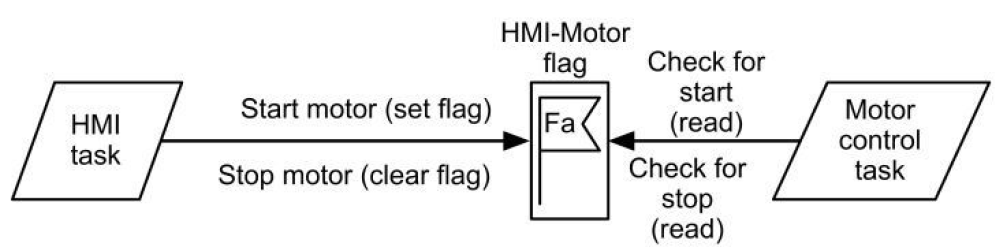
\includegraphics{Chapter5/simple_flag1.PNG}
        \caption{Simple flag implementation}
        \label{fig:simple_falg1}
    \end{figure}
    At the code level, flags are binary items.
    Code implementation :
    
    \texttt{typedef enum $\{$Start, Stop$\}$ StartStopFlag;}
    
    \texttt{StartStopFlag HMImotorFlag = Stop;}

    A more secure design is one where each individual command has a corresponding flag: One motor start flag and one motor stop flag. (this introduces some redundancy in the information). 
    The rules used here are that:
    \begin{itemize}
        \item The HMI sending task checks to see that a flag is reset before changing its state. 
        \item The Motor control task checks the state of both flags before acting on a command. After a successful check, the commanding flag is then reset. 
    \end{itemize}
    
    \begin{figure}[H]
        \centering
        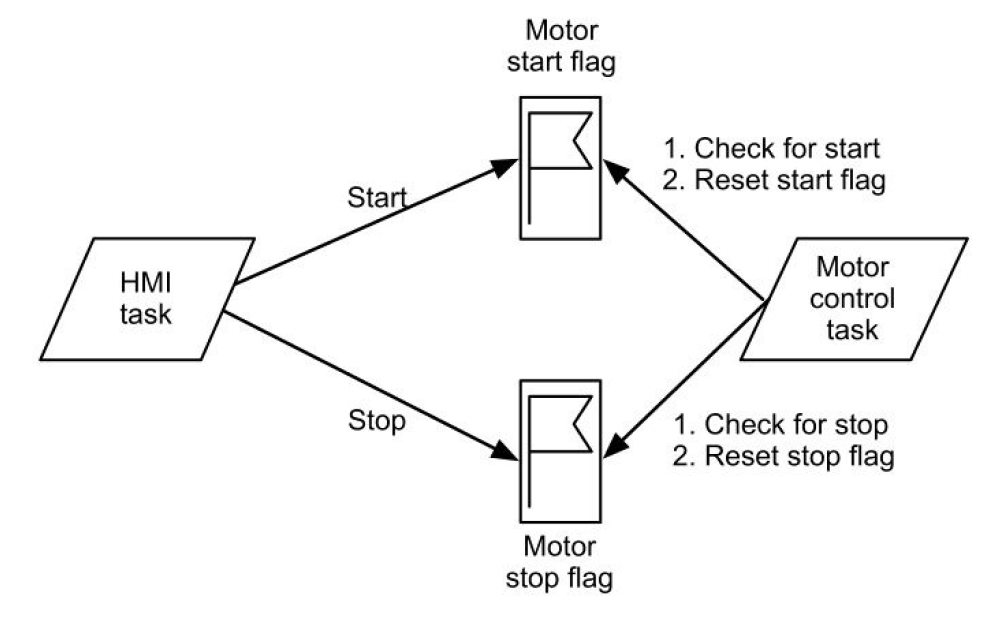
\includegraphics{Chapter5/simple_flag2.PNG}
        \caption{Improved use of flags}
        \label{fig:simple_falg2}
    \end{figure}
    
     \vspace{5pt} \hrule
    \item \textbf{Explain the "conditions flag group" mechanism for task interaction without data transfer (in 1-page !)}
    
    \begin{figure}[H]
        \centering
        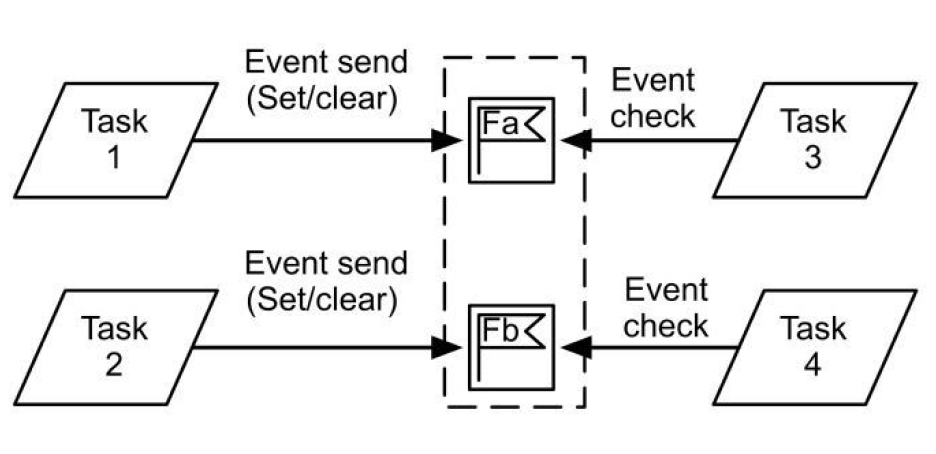
\includegraphics{Chapter5/group_flag1.PNG}
        \caption{Condition flag group implementation}
        \label{fig:group_falg1}
    \end{figure}
    
    Condition flag group = group where we group a set of flags together into a single unit. The flag group is a single word, each flag being a bit within the word. As a result: 
    \begin{itemize}
        \item Each bit can be changed individually 
        \item The whole group can be modified using a single write command
        \item Sets of bits can be changed using bit masking techniques.
    \end{itemize}
    Especially useful : 
    \begin{itemize}
        \item where a task is waiting on a set of events: Easier to implement combinational logic operation (logical AND/OR)
        \item where a task broadcasts an event to a number of other tasks 
    \end{itemize}
    
    \begin{figure}[H]
        \centering
        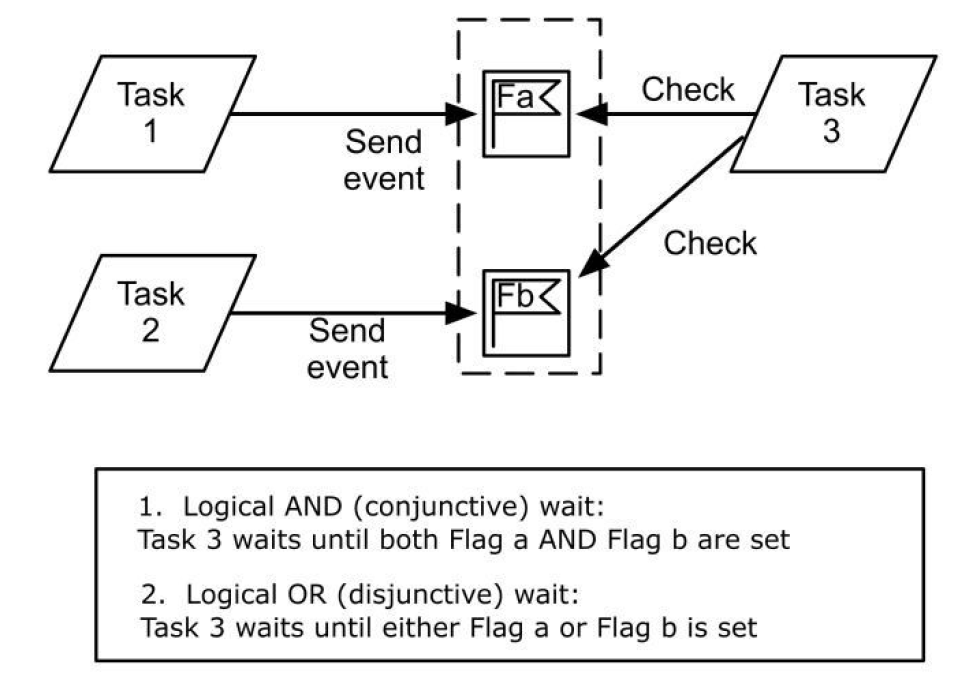
\includegraphics{Chapter5/group_flag2.PNG}
        \caption{Waiting on a set of events}
        \label{fig:group_falg2}
    \end{figure}
    
    \begin{figure}[H]
        \centering
        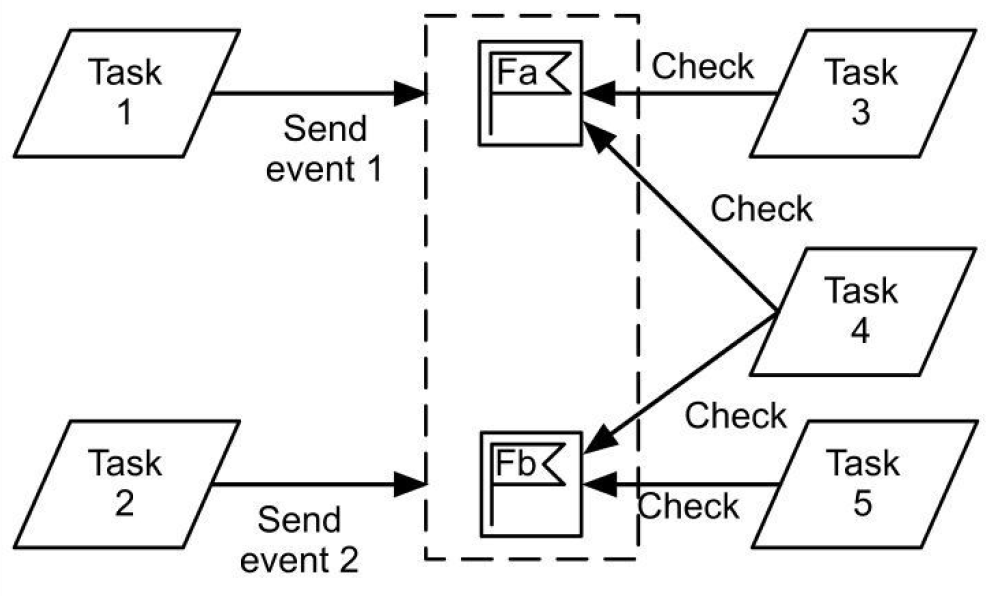
\includegraphics{Chapter5/group_flag3.PNG}
        \caption{Broadcast function}
        \label{fig:group_falg3}
    \end{figure}
    
     \vspace{5pt} \hrule
    \item \textbf{Explain the "unilateral rendez-vous" mechanism for task synchronization using event flags (in 1-page !)}
    
    The unilateral ('one-way') rendezvous is a limited form of synchronization. 
    
    \begin{figure}[H]
        \centering
        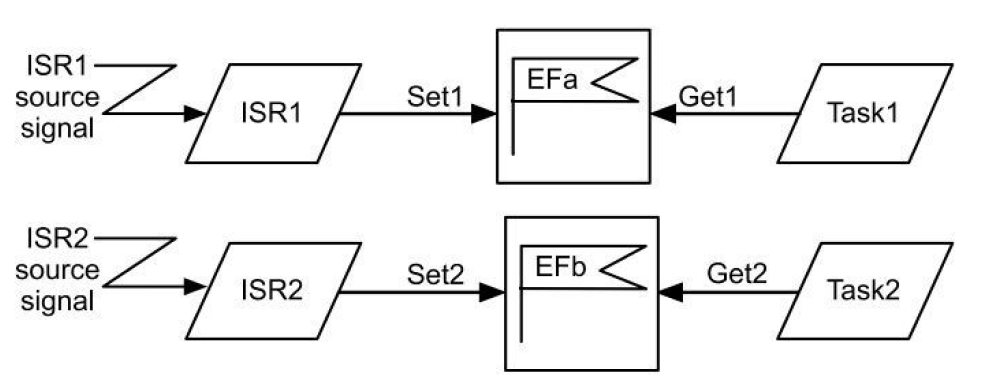
\includegraphics{Chapter5/unilateral_rendezvous.PNG}
        \caption{Unilateral synchronization}
        \label{fig:unilateral}
    \end{figure}
    
    Here event flags are used to support task-to-task interaction, the basic rules being:
    \begin{itemize}
        \item ISR1(2) is a sender task. Task1(2) is its corresponding receiver.
        \item The event flag is initialized to the cleared state (flag value = 0).
        \item When a task calls Get on a cleared flag it is suspended.
        \item When a task calls Get on a set flag (flag value = 1) it clears the flag and continues executing.
        \item When a task calls Set on a cleared flag, it sets that flag and continues executing. If a task is waiting suspended on that flag it is woken up (readied).
        \item When a task calls Set on a set flag it just continues executing.
    \end{itemize}
    
    For the example of Figure \ref{fig:unilateral}:
    \begin{itemize}
        \item If Task1 calls 'Get1' before ISR1 has generated 'Set1', it is suspended. When 'Set1' is subsequently sent to the flag (EFa), Task1 is readied.
        \item If 'Set1' is generated before Task1 calls 'Get1' (i.e. the ISR task reaches the synchronization point first), ISR1 does not stop but continues execution. However the Set call leaves flag EFa in the set state. As a result, when task 1 calls Get, it first clears the flag and then carries on executing.
    \end{itemize}
    
     \vspace{5pt} \hrule
    \item \textbf{Explain the "bilateral rendez-vous" mechanism for task synchronization using signals (in 1-page !)} 
    
    Such synchronization is achieved by using signals, these being 'Wait', 'Send' and 'Check'.
    
    \begin{figure}[H]
        \centering
        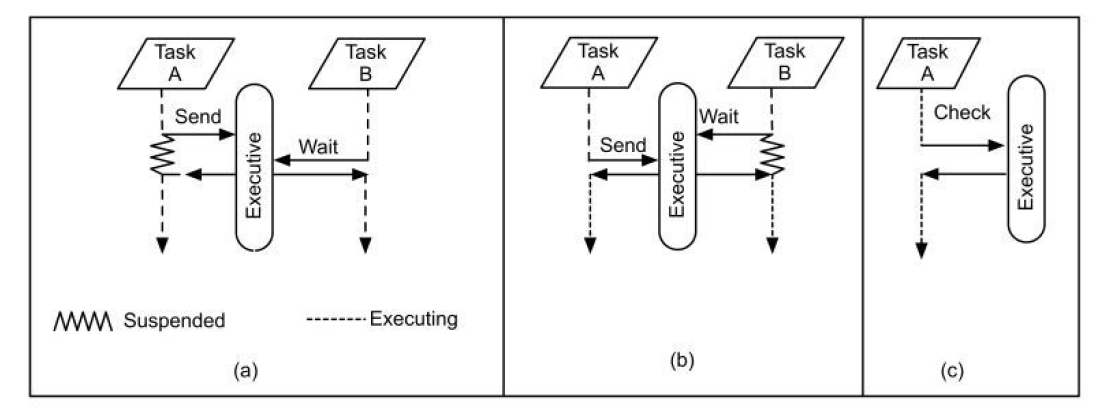
\includegraphics{Chapter5/bilateral_rendezvous.PNG}
        \caption{Bilateral synchronization}
        \label{fig:bilateral}
    \end{figure}
    Signalling activities are the responsibility of the executive.
    
    First consider the 'Send' action, Figure \ref{fig:bilateral}(a). Here task A executes its program and reaches a point where it sends a signal (effectively to the executive). At that instant no tasks are waiting to receive this signal; consequently task A is suspended. Some time later task B generates a wait request for the signal sent by A. It (task B) picks up the signal and carries on executing. The wait request also restarts Task A.
    
    What happens if B generates the wait before A has sent the signal, Figure \ref{fig:bilateral}(b)? The result; task B is suspended until A sends the signal. At this point task A wakes task B and then continues executing.
    
    Flexibility can be added to the signal construct by allowing tasks to decide if they wish to get involved in synchronization. The Check operation, Figure \ref{fig:bilateral}(c), surveys the status of the signal but does not itself halt task execution. Such decisions are left to the checking task, a technique that can be used very effectively for polling operations.
    
    \begin{enumerate}[label=(\roman*)]
        \item There isn't a one-to-one link between tasks; task pairing is not specified in these constructs.
        \item Tasks are considered to be both senders and receivers.
        \item Signals aren't associated with specific tasks. All that is required that one task has the Wait whilst the other has the corresponding Send.
        \item They exhibit the insecurities of the semaphore.
        \item Signals look remarkably like binary semaphores, something which causes great confusion. In fact their implementations are very similar. The fundamental difference is in how they are used, not their construction. Semaphores are generally used as mutual exclusion mechanisms, signals for synchronization.
        \item Few RTOSs provide the bilateral synchronizing construct.
    \end{enumerate}
    
    Semaphores may be used to create signals, but there isn’t a simple one-to-one relationship. One design method employs two semaphores (one for each direction of signalling , Figure \ref{fig:bi_semaphore}) to build a single signal.
    
    \begin{figure}[H]
        \centering
        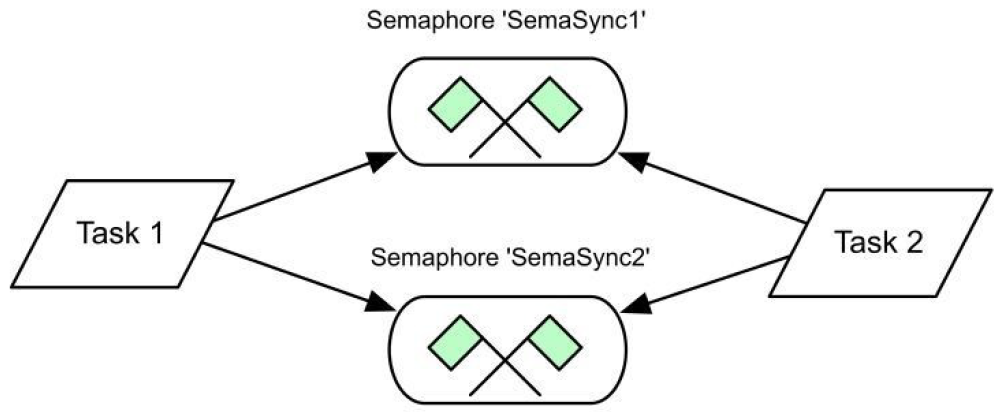
\includegraphics{Chapter5/bilateral_semaphore.PNG}
        \caption{Signal implementation using semaphore}
        \label{fig:bi_semaphore}
    \end{figure}
    
    In practice, it is much better practice to use monitor-type techniques, giving conceptually the structure of Figure \ref{fig:bi_monitor}.
    
    \begin{figure}[H]
        \centering
        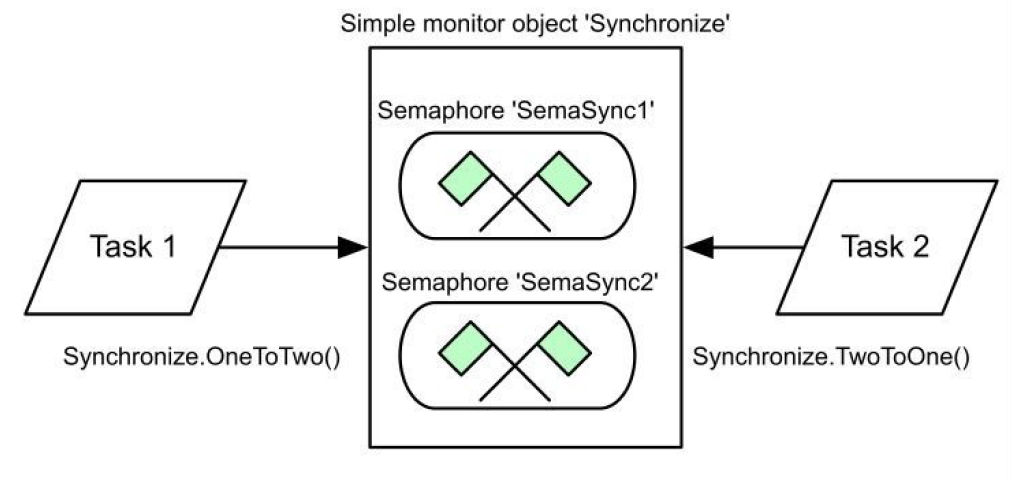
\includegraphics{Chapter5/bilateral_monitor.PNG}
        \caption{Signal implementation using monitor}
        \label{fig:bi_monitor}
    \end{figure}
    
     \vspace{5pt} \hrule
    \item \textbf{Explain the "Queues" mechanism for data transfer without task synchronization (in 1-page !)} 
    
    Queues are used as communication pipes between processes, normally on a one-to-one basis (Figure \ref{fig:queue1}). 
    
    \begin{figure}[H]
        \centering
        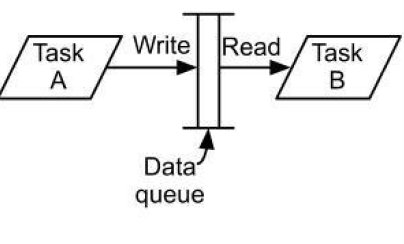
\includegraphics{Chapter5/Queue1.PNG}
        \caption{Sequential access}
        \label{fig:queue1}
    \end{figure}
    
    Here, task A deposits information into the queue, task B extracting it in first-in first-out style. The queue is usually made large enough to carry a number of data words, not just a single data item. As such it acts as a buffer or temporary storage device, providing elasticity in the pipe. Its advantage is that insertion and extraction functions can proceed asynchronously (as long as the pipe does not fill up). It is implemented in RAM.
    
    The linked list structure has a very useful feature is that its size is not necessarily fixed, but can be expanded or contracted as desired. Further, very large queues can be built, limited only by the available memory space. But first, if RAM is limited, it is impossible to construct large queues at all. Second, large FIFO queues handling multiple messages can have a long transport delay from data-in to data-out. The resulting performance may be too slow for many real-time applications. $\Rightarrow$ Not appropriate for embedded systems.
    
    A circular buffer is normally assembled using a fixed amount of memory space, Figure \ref{fig:queue2}(a), being designed to hold a number of data units. What makes the queue circular is that data unit 0 is the successor of data unit 9; addressing is done using modulo 9 counting.
    
    Figure \ref{fig:queue2}(b) shows how pointers are used to identify the start and finish locations of the stored data ('Reader' and 'Sender'). By using these we do not have to shift data through the buffer. Inserted data units always stay in the same memory locations; only the pointers change value - as demonstrated in Figures \ref{fig:queue2} (c) and (d). These pointers can also be used to define the 'queue full' and 'queue empty' conditions - they become equal.
    
    Under normal circumstances tasks A and B proceed asynchronously, inserting and removing data from the queue as required. Task suspension occurs only under two conditions, queue full and queue empty.
    
    \begin{figure}[H]
        \centering
        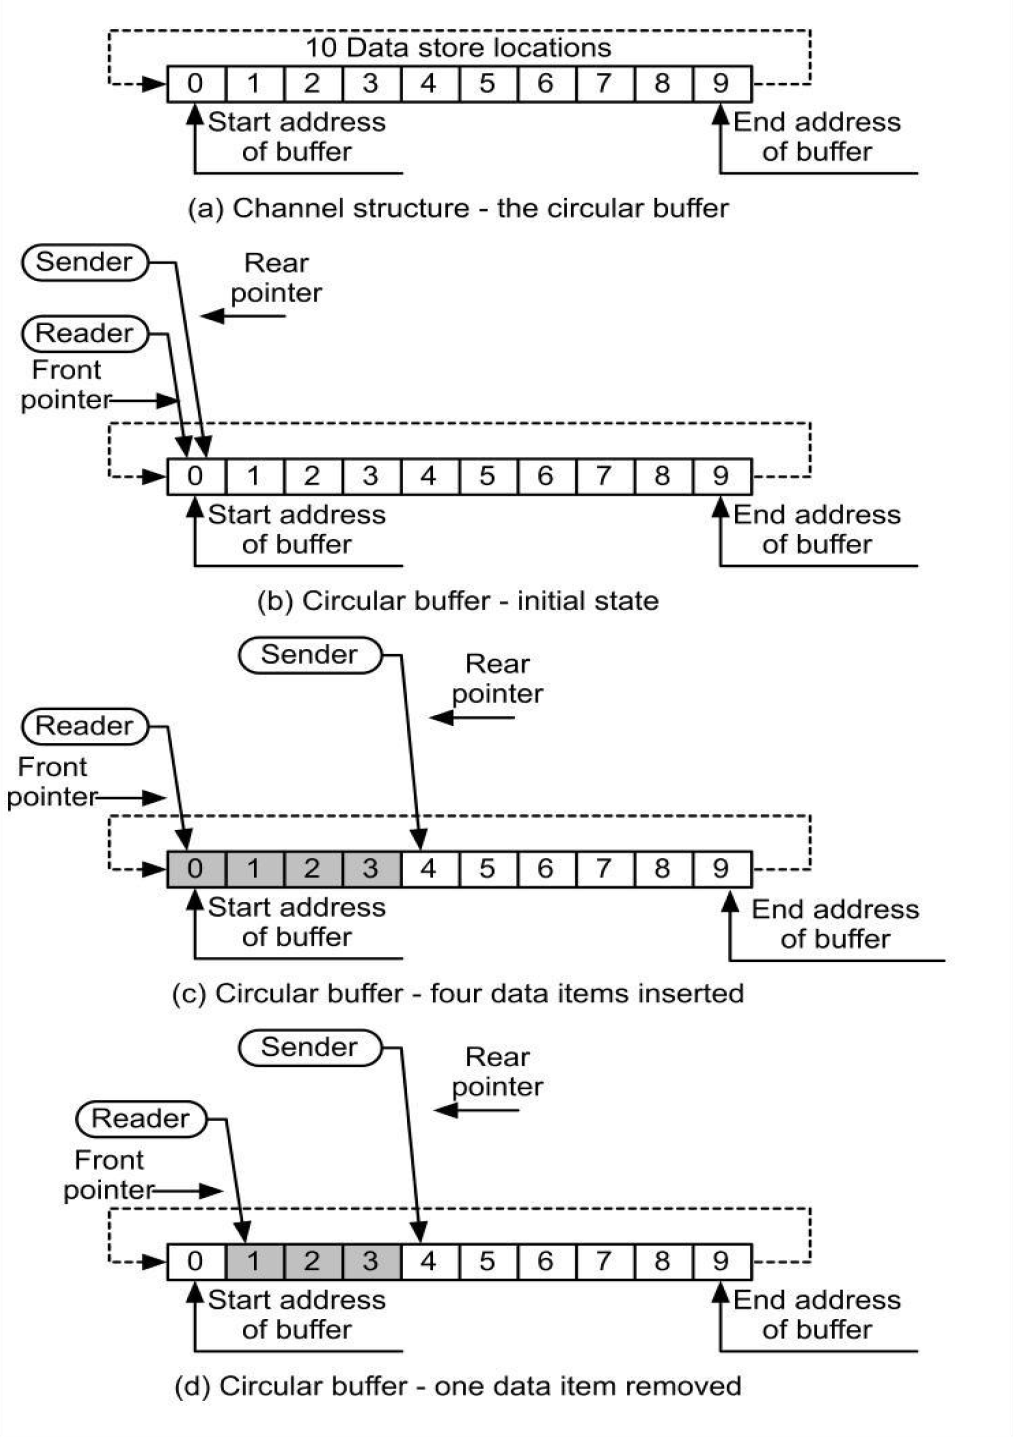
\includegraphics{Chapter5/Queue2.PNG}
        \caption{The circular buffer}
        \label{fig:queue2}
    \end{figure}
    
     \vspace{5pt} \hrule
    \item \textbf{Explain the "Mailbox" mechanism for data transfer with task synchronization (in 1-page !)} 
    
    The mailbox incorporating signals for synchronization and storage for data, Figure \ref{fig:mailbox}.
    
    \begin{figure}[H]
        \centering
        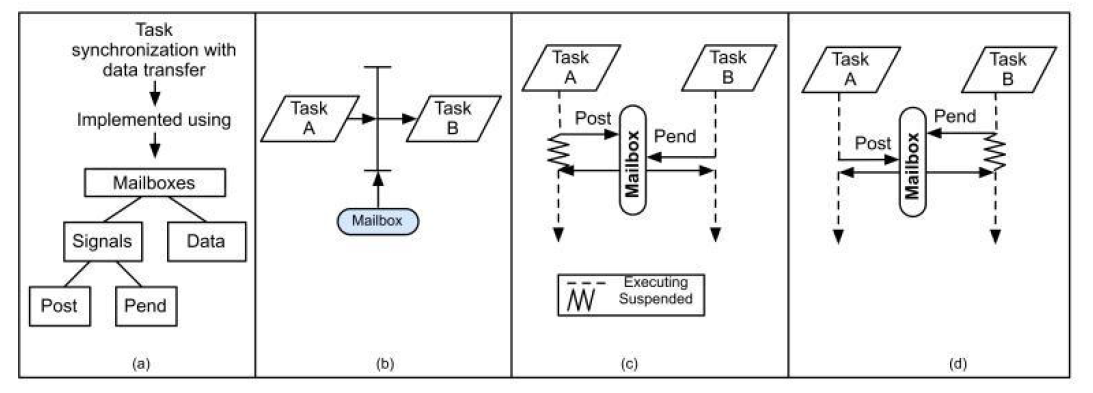
\includegraphics{Chapter5/mailbox.PNG}
        \caption{Data transfer with task synchronization}
        \label{fig:mailbox}
    \end{figure}
    
    When a task wishes to send information to another one it 'posts' the data to the mailbox. Correspondingly, when a task looks for data in the mailbox it 'pends' on it. In reality, Post and Pend are signals. Moreover, the data itself is not normally passed through the mailbox; a data pointer is used. Even so, no matter how large the data contents are, the data is treated as a single unit.
    
    Task synchronization is achieved by suspending or halting tasks until the required conditions are met, Figures \ref{fig:mailbox} (c),(d).
    
    \vspace{5pt} \hrule
    
\end{enumerate}

\newpage

\section{Chapter 6: \textit{Memory usage and management}}

\begin{enumerate}
    \item \textbf{Explain the different types of non-volatile memory devices} 
    
    There are three categories of non-volatile store, depending on how information can be reprogrammed.
    
    \begin{figure}[H]
        \centering
        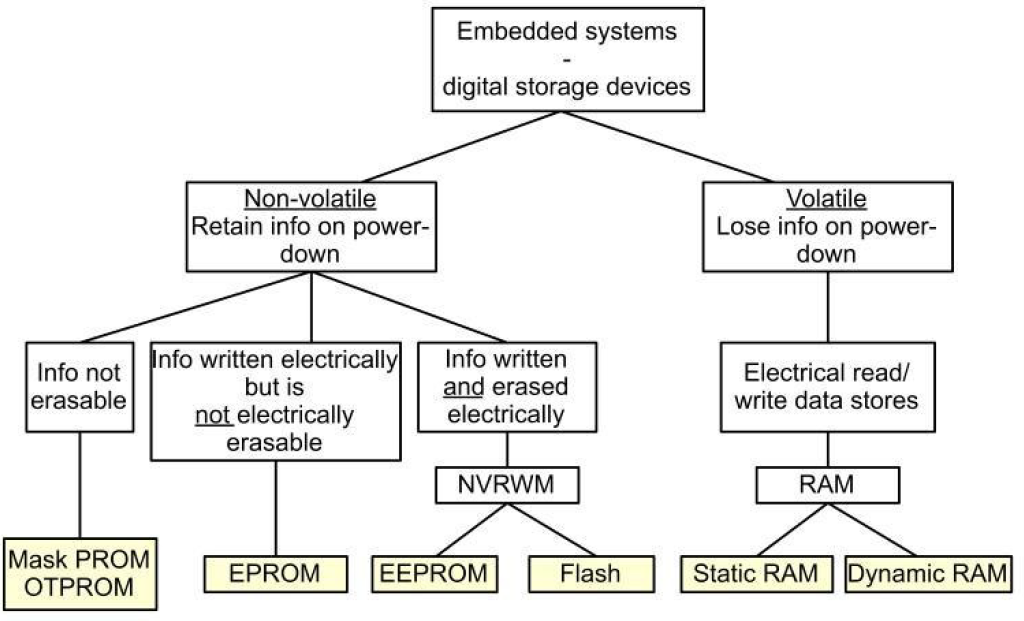
\includegraphics{Chapter6/Non_volatile.PNG}
        \caption{Memory device in embedded systems}
        \label{fig:memory_devices}
    \end{figure}
    
    \begin{enumerate}
        \item \textbf{Non-erasable storage}\\
        There are two types of non-erasable storage devices, the mask programmable read-only memory (mask PROM) and the one-time programmable read-only memory (OTPROM). Mask PROMS, which are programmed during manufacture, are the cheapest of all provided very large numbers are used. OTPROMs are supplied in the erased state and are then programmed electrically by the user. The programmed data cannot subsequently be changed, and is retained indefinitely by the device.
        \item \textbf{UV erasable storage - EPROM}\\
        The next device to consider is the UV-erasable electrically programmable readonly memory (EPROM). Here the device contents are erased using ultra-violet light, whilst writing new information is done electrically. To change the stored information the EPROM is first erased, then re-programmed with the new material.
        \item \textbf{Non-volatile read-write memories - NVRWM}\\
        The third group are the non-volatile read-write memories, NVRWM, consisting of two technologies. The first is the electrically erasable programmable ROM (EEPROM), the second being Flash memory. With these, erasure and (re)programming is done electrically; any other differences aren't of particular interest to us at this stage. Flash memory is widely used in single-chip microcontrollers, so much so that the word Flash tends to be used as a generic term (aka Hoover for vacuum cleaner). Other devices in this category include the ferro-electric random access memory (FRAM) and the magnetoresistive RAM (MRAM). At this time they aren't yet widely used in embedded systems.
    \end{enumerate}
    
    \vspace{5pt} \hrule
    
    \item \textbf{Explain why task interference can occur and how MPUs and MMUs are used to prevent such interferences (in 1-page)} 
    
    The distinction between private and shared (public) memory is merely conceptual. There is absolutely no reason why task 1, for instance, cannot access the private memory of tasks 2 and 3. This points up the need for some form of protection mechanism.
    \begin{itemize}
        \item \textbf{Controlling memory accesses with a memory protection unit (MPU)}\\
        A hardware device specifically designed to prevent tasks making invalid memory accesses is the memory protection unit (MPU). It is programmed to hold task address information, specifically the address limits.
        
        \begin{figure}[H]
            \centering
            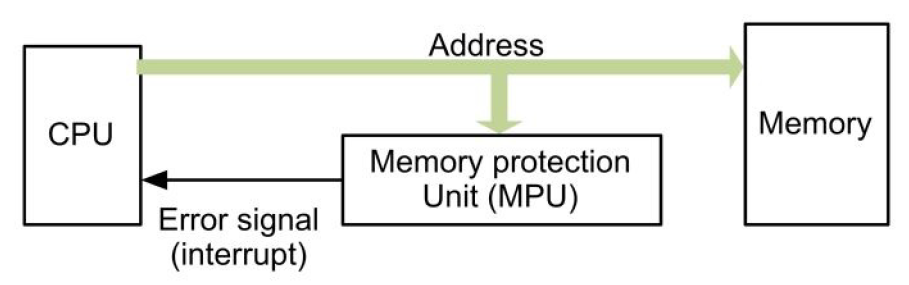
\includegraphics{Chapter6/MPU.PNG}
            \caption{MPU}
            \label{fig:mpu}
        \end{figure}
        
        The MPU monitors the address information flowing between the CPU and the processor memory; any violation of address bounds causes an error signal (exception) to be produced. 
        
        The MPU can be looked at from two points of view: processor level and task level, Figure \ref{fig:mpu_prot}.
        
        \begin{figure}[H]
            \centering
            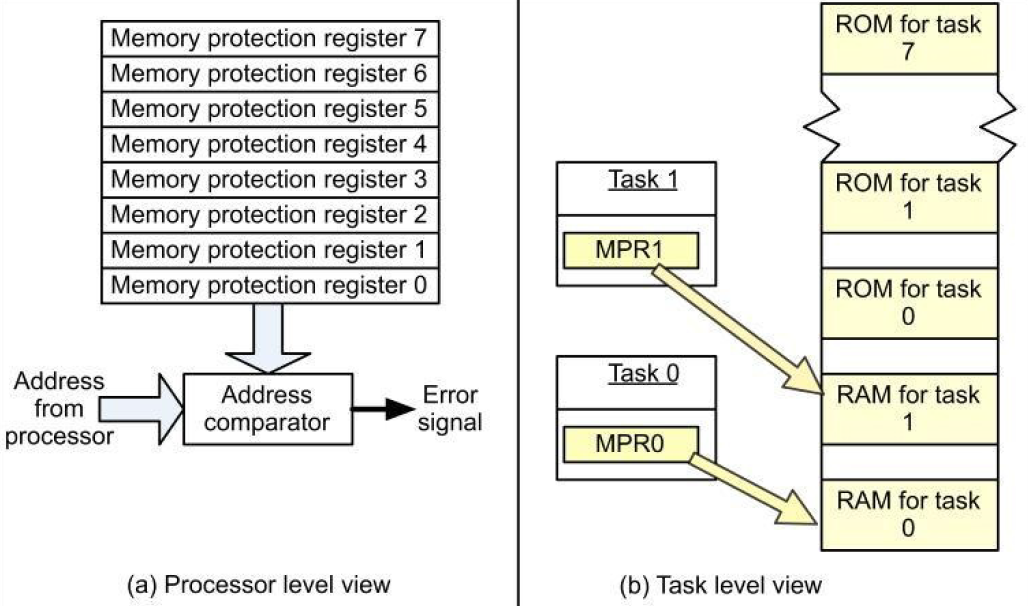
\includegraphics{Chapter6/MPU_prot.PNG}
            \caption{Example of physical memory structure}
            \label{fig:mpu_prot}
        \end{figure}
        
        Central to the protection scheme is a set of memory protection registers (MPRs). The example here has eight registers, each one holding the memory address bounds of a task (base address plus associated range size). At task creation time each protection register is configured with the appropriate memory information. During task execution each address generated by the processor is compared with those held by its MPR; any attempt to access memory outside of the predefined limits raises an exception. In this example protection is provided for RAM areas only; some MPUs also have code protection registers.
        
        \item \textbf{Controlling memory accesses with a memory management unit (MMU)} In some exeptions, systems intended to support multiple software applications. Applications like these frequently run on micros that have different memory sizes and configurations. Information about the target memory structure, the physical memory, isn't known at compile time.
        
        Programmers can then decide what addresses they wish to use for any particular application. These are called the 'logical' addresses, and are the ones seen by the processor. However, these logical values cannot be applied directly to the real memory; they must first be mapped into the memory address space, the 'physical' addresses.
        
        So, the MMU contains a set of translation registers that are used to convert the logical addresses (those generated by the CPU) to the physical ones (those seen by the memory). These registers are re-loaded with translation data when the new application software is loaded into main memory. A secondary role of the MMU is that of memory protection. It executes this function in exactly the way as that of the MPU described earlier.
        
        \begin{figure}[H]
            \centering
            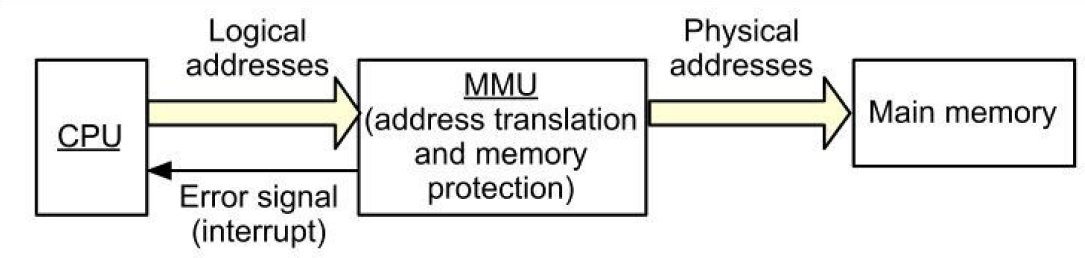
\includegraphics{Chapter6/MMU.PNG}
            \caption{The role of MMU}
            \label{fig:mmu}
        \end{figure}
        
    \end{itemize}
    
    \vspace{5pt} \hrule
    
    \item \textbf{Explain the difference between static and dynamic memory allocation techniques}
    
    \begin{itemize}
        \item \textbf{Static} The amount and location of RAM provided for each task is define in the code by the programmer. Or the decision is left to the compiler. So the decision will remains unchanged during the lifetime of the task. 
        \item \textbf{Dynamic} The system to allocate RAM only when it is needed; on completion of the required activities it is retrieved for future use ('deallocated').
        
        \begin{figure}[H]
            \centering
            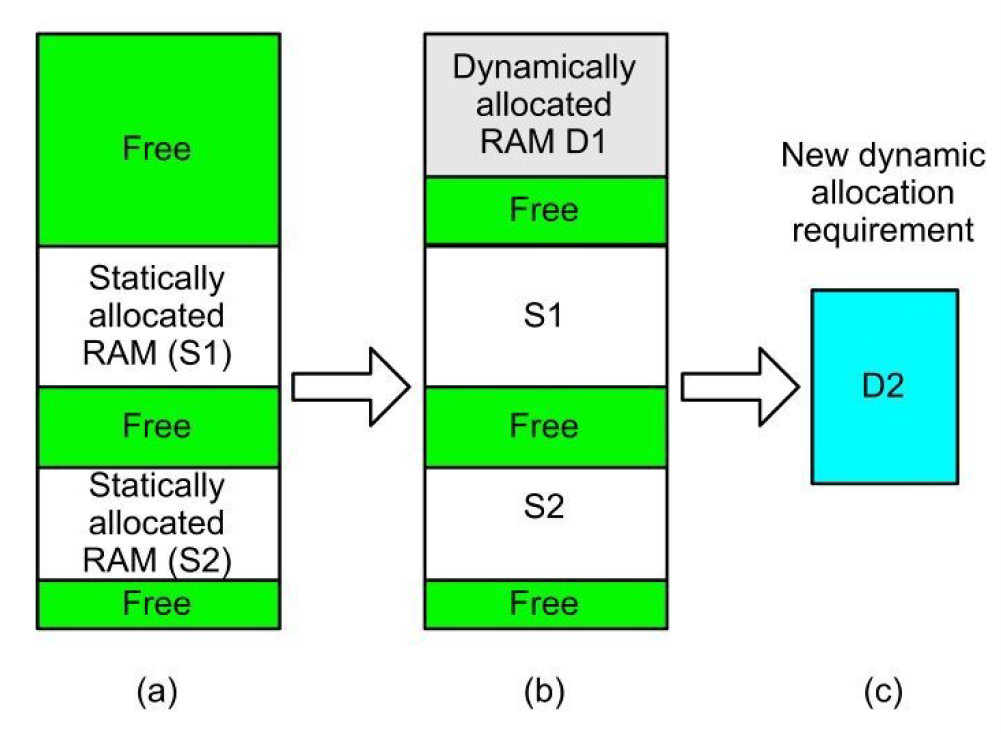
\includegraphics{Chapter6/Static_dyna_alloc.PNG}
            \caption{Memory allocation, fragmentation and its consequences}
            \label{fig:stat_dyna}
        \end{figure}
    \end{itemize}
    
    \vspace{5pt} \hrule
    
    \item \textbf{Explain why dynamic memory allocation can result in memory fragmentation and leakage (in 1-page)} 
    \begin{itemize}
        \item \textbf{Fragmentation} Because the dynamically allocated memory is not nicely, compactly, organised; instead it is fragmented throughout the available memory space. Some day a task will request an allocation of memory greater than any of the free areas, figure \ref{fig:stat_dyna}(c).
        \item \textbf{Leakage} Figure \ref{fig:leakage}(a) shows a situation where a static memory allocation has been made for two tasks, T1 and T2. Task 1 uses memory area S1, task 2 using area S2. Let's assume that at some later stage, figure \ref{fig:leakage}(b), task 1 invokes a function which calls malloc(), to dynamically acquire extra memory, D1. Unfortunately, owing to a programmer mistake, the function terminates without calling free(); thus it doesn't deallocate D1. As a result the amount of free memory is now permanently reduced for the duration of the program. We have 'leaked' memory from the available pool.
        
        \begin{figure}[H]
            \centering
            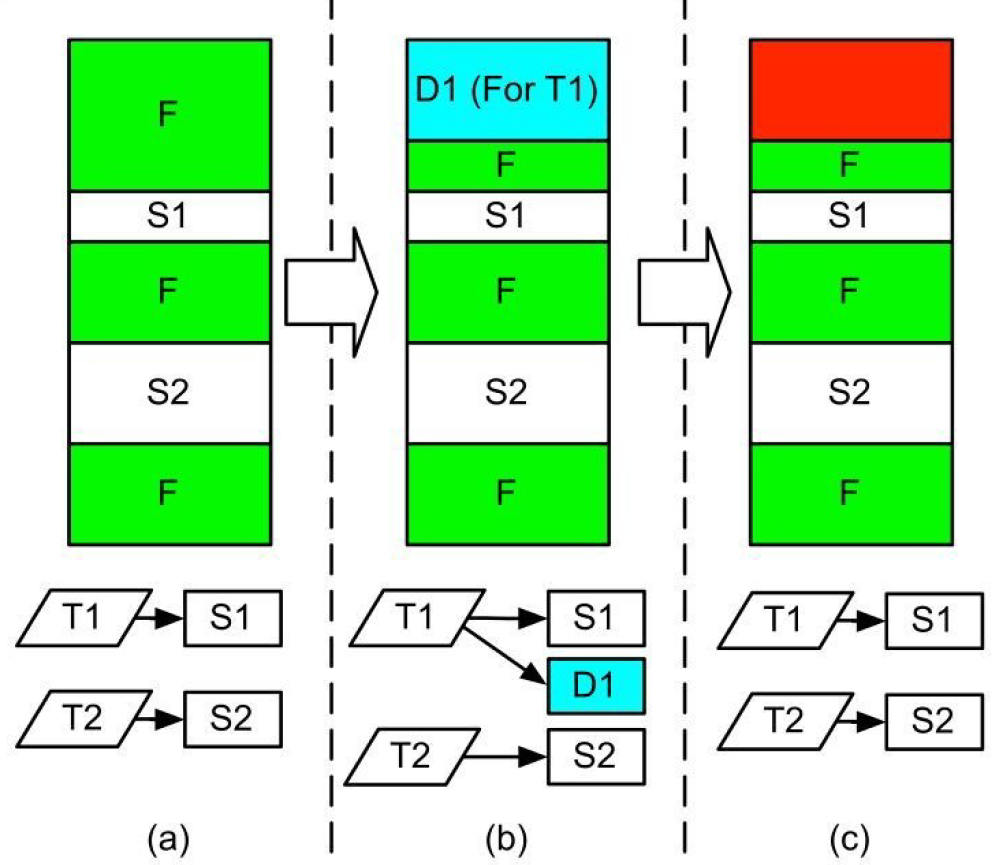
\includegraphics{Chapter6/Leakage.PNG}
            \caption{Memory allocation, Leakage and its consequences}
            \label{fig:leakage}
        \end{figure}
        
    \end{itemize}
    
    \vspace{5pt} \hrule
    
    \item \textbf{Explain the "Secure memory allocation" technique (in 1-page)}
    
    First, we have to find out exactly how much RAM we have in our embedded system. Second, we decide what memory, and how much of it, we will use for dynamic operations.
    We then split the dynamic allocation into 'partitions' (or 'pools') which have fixed positions in the memory map. Each partition is, in turn, formed as a series of 'blocks', all blocks being located at fixed addresses.
    As shown here, the rules for memory allocation and deallocation are simple and straightforward.
    \begin{itemize}
        \item Memory is allocated from selected partitions.
        \item Only one block is allocated for each request made.
        \item A count is held of the number of blocks currently allocated.
        \item Deallocated memory is always returned to the partition it came from in the first case.
        \item Only one block is returned for each return request made.
        \item Allocation/deallocation times are deterministic.
        \item Errors are flagged up if an allocation request is made to an empty partition or if a return is attempted to a full partition.
    \end{itemize}
    
    \begin{figure}[H]
        \centering
        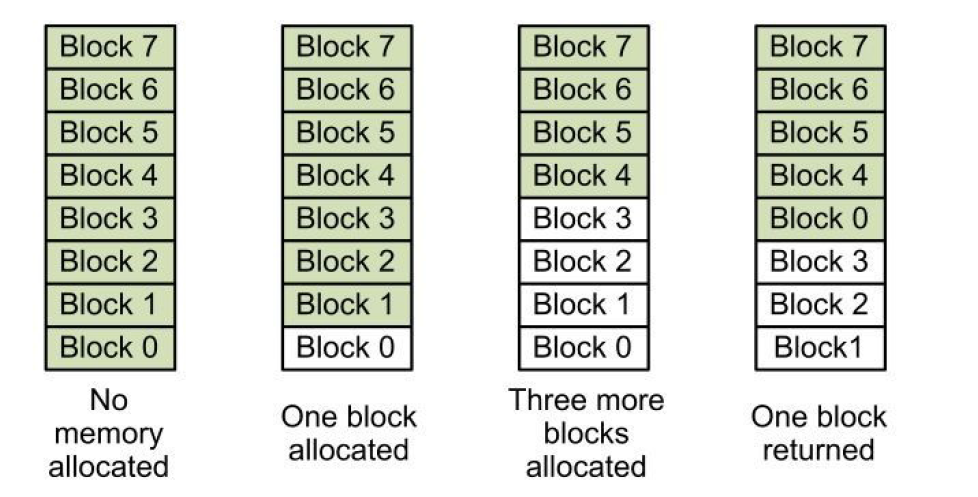
\includegraphics{Chapter6/Secure_alloc.PNG}
        \caption{Memory block allocation and deallocation}
        \label{fig:secure_alloc}
    \end{figure}
    
    To make this work in practice, we use what is generally called a 'memory control block', Figure \ref{fig:memory_blocks}.
    
    \begin{figure}[H]
        \centering
        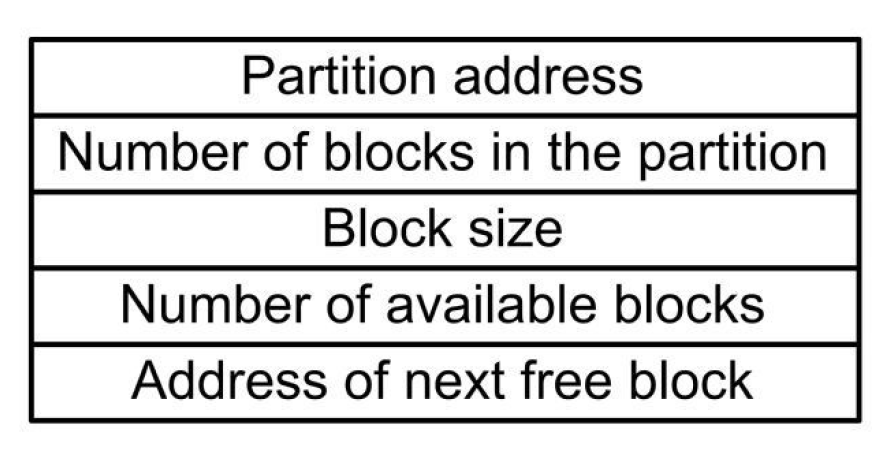
\includegraphics{Chapter6/Memory_block.PNG}
        \caption{The memory (partition) control block}
        \label{fig:memory_blocks}
    \end{figure}
    
    Key to the reordering of blocks is the use of address (pointer) techniques to create a linked list of memory locations. This makes it quite easy to reorder the logical arrangement of the physical memory blocks.

    \vspace{5pt} \hrule
    
\end{enumerate}

\newpage

\section{Chapter 7: \textit{Multiprocessor systems}}

\begin{enumerate}
    \item \textbf{Explain the symmetric and asymmetric types for multicore processors. Give an example of block diagram for each of them.}
    \begin{itemize}
        \item \textbf{Symmetric} The ARM Cortex A9, figure \ref{fig:sym} showing a simplified description of its key features. It has four identical processing units (cores), each one consisting of a CPU, hardware accelerator, debug interface and cache memory. It can be seen that several on-chip resources are shared by all the processing units. From a software perspective the device can be used in two ways. First, each core can be allocated specific tasks, and hence is considered to be a dedicated resource. Second, any core can run any task, thus being treated as an anonymous resource.
        
        \begin{figure}[H]
            \centering
            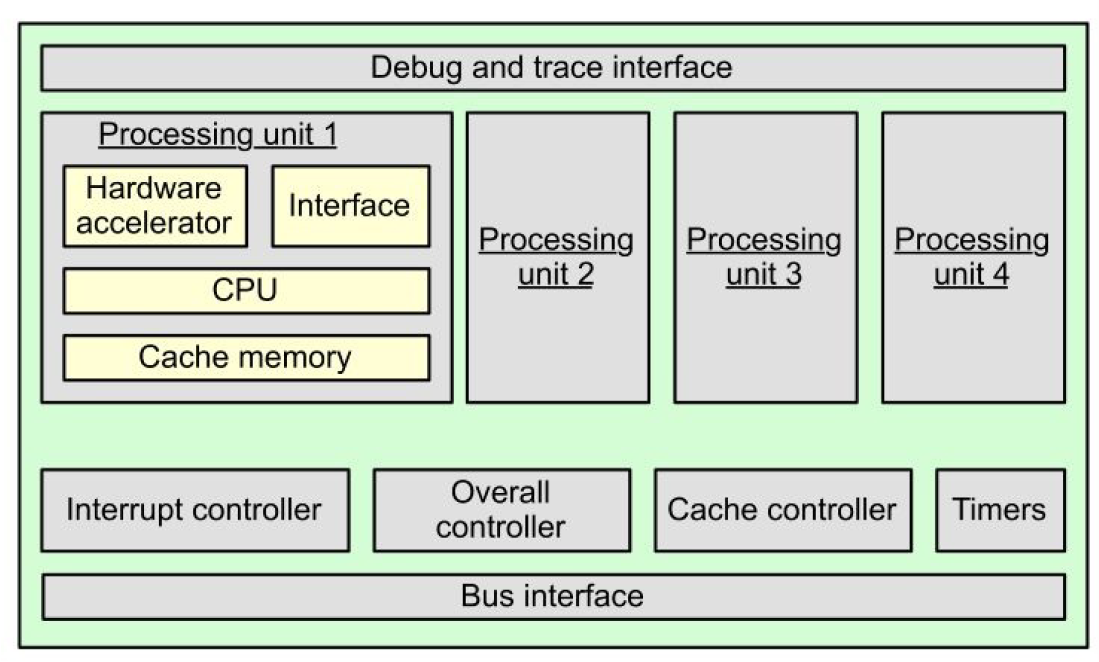
\includegraphics[scale=0.9]{Chapter7/Sym.PNG}
            \caption{Example symmetric multiprocessor - multicore implementation}
            \label{fig:sym}
        \end{figure}
    
        \item \textbf{Asymmetric} The Texas TMS320DM6443, figure \ref{fig:asym}. In this device there are two distinct processing units, one for general purpose computing and the other for digital signal processing. Generally, multicore processors are organized as single-board computing elements. These may be part of a complete single-board computer or else form the single processing unit of multi-board designs. Either way they can be viewed as being equivalent to very high performance single core devices, quite different to multi-board multicomputer structures.
    
        \begin{figure}[H]
            \centering
            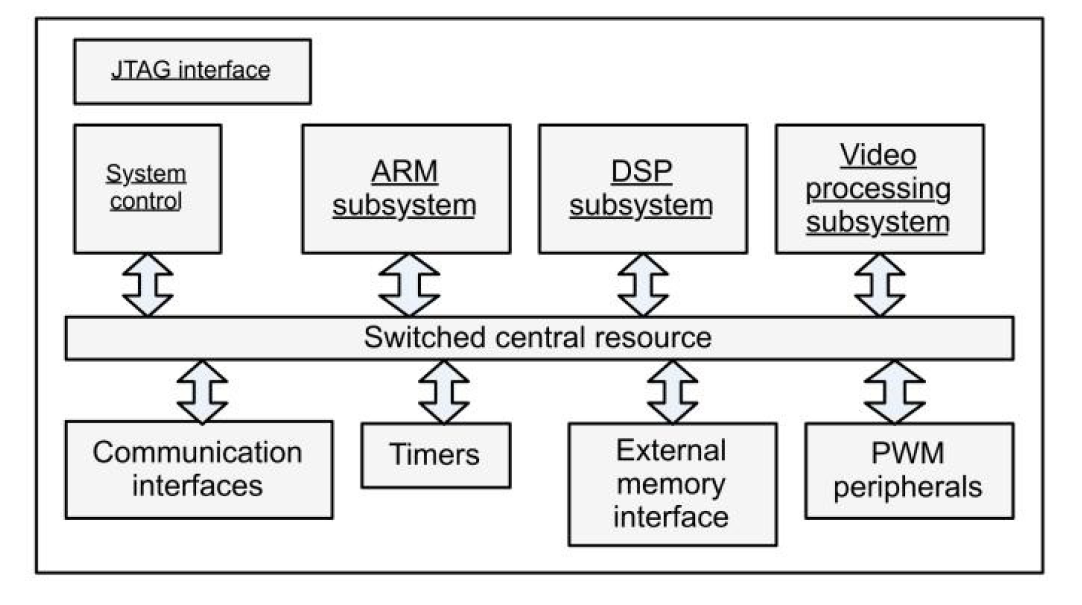
\includegraphics[scale=0.9]{Chapter7/Asym.PNG}
            \caption{Example asymmetric multiprocessor - multicore implementation}
            \label{fig:asym}
        \end{figure}
        
    \end{itemize}
    
    \vspace{5pt} \hrule
    
    \item \textbf{Explain what is meant by AMP, SMP, BMP and mixed-mode systems. Give their relative advantages and disadvantages.}
    
        \begin{figure}[H]
            \centering
            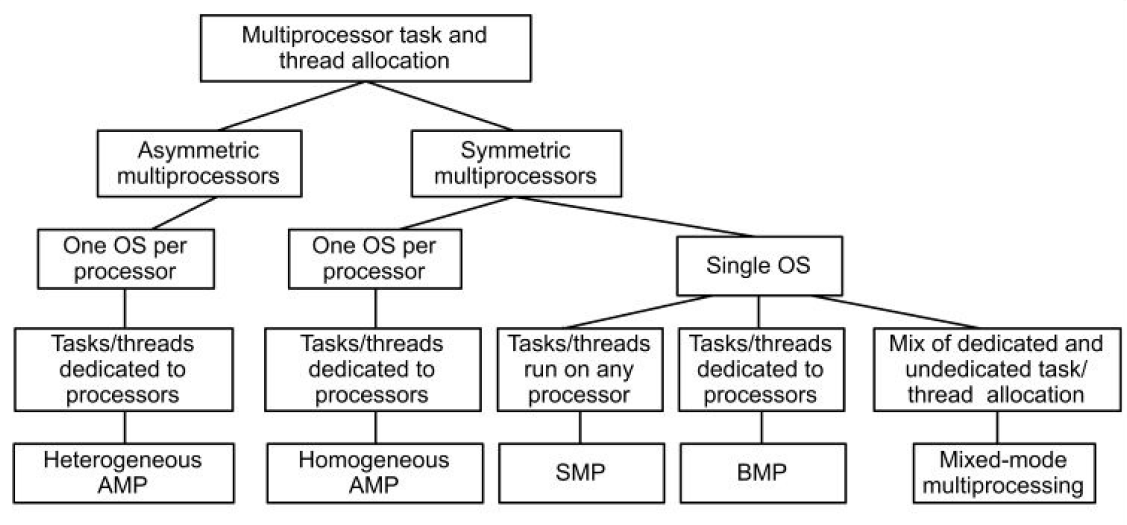
\includegraphics{Chapter7/Multi_processor.PNG}
            \caption{Multiprocessor task and thread allocation}
            \label{fig:multi}
        \end{figure}
        
        \begin{itemize}
            \item \textbf{AMP} systems behave like a set of collaborating microcomputers sharing a predefined set of resources such as memory, interrupts and peripherals. Because each micro has its own OS, the designer is not limited to a single scheduling technique (this is true of both multicore and multicomputer designs).
            
            The designer normally determines the allocation and use of the various resources, and does this explicitly. Such information is 'hard-wired' into the source code, being executed during processor initialization. Generally, for embedded applications, resources aren't dynamically reallocated during program execution.
            
            \textit{Advantages:} AMP systems give us improved performance without sacrificing the determinism, predictability and security of the single core RTOS. Moreover, it is relatively straightforward to port an existing single-processor design to an AMP system.
            
            \textit{Disavantages:} Because the processors have dedicated tasks, individual processor loadings (hence utilization) may, in practice, be quite different. This limits the speed-up advantages of an AMP design.
            \item \textbf{SMP} The key feature, the whole purpose, of SMP systems is to deliver high performance by keeping all the processor fully utilized. The key to this is to:
            \begin{itemize}
                \item Have one OS only
                \item Allow this OS to see the whole system
                \item Enable the OS to dynamically control the allocation of tasks/threads to micros
                \item Permit the OS to allocate and control the use of system resources
            \end{itemize}
            For example, consider programming the algorithm
            $$y = F_0(x_0) + F_1(x_1) + F_2(x_2) + F_3(x_3)$$
            for a four-core device using Pthreads.
            \begin{itemize}
                \item Creation of four threads
                \item Execution of the code of the individual threads
                \item Synchronization of the completed threads
            \end{itemize}
            Here we have a classic solution to the need to program a set of essentially independent parallel, repetitive calculations. In this case it doesn't matter which cores the threads run on.
            
            \textit{Advantages:} The programmer plays no part in deciding where the threads should run. He does not need to consider low-level detailed activities. The code is also highly portable; for example, there is no need to change the source code to run it on a two-core device. Another advantage is the flexibility of the implementation technique; exactly the same approach could be used for (say) an eight-thread filter implementation.
            
            \textit{Disavantages:} Not suitable for embedded applications because:
            \begin{itemize}
                \item It is often impossible to predict the execution order of individual threads, even with a priority pre-emptive scheduler. If execution order is important (e.g. for coordination purposes) the code must be explicitly designed to guarantee that this will happen.
                \item It is impossible to predict on which core the processes will run. When the software is flawless this isn't an issue; the same isn't true when bugs are present.
                \item Real-time behaviour may not be guaranteed for some processes. For example, in a single processor system a high priority interrupt service routine will always pre-empt normal scheduled threads. This ensures that there can be no conflict between the two. However, in a multicore design the ISR could be executed on one core whilst the others continue to run the scheduled threads.
                \item Taken together, these factors can be important when porting an existing single processor design to a multiprocessor system. Synchronization, coordination and exclusion properties may not be maintained.
            \end{itemize}
            
            \item \textbf{BMP}
            
            With BMP you can specify which processors the tasks/threads should run on.
            
            \textit{Advantages:} Provides high degree of predictable behaviour. Which is very useful for critical software.
            
            \textit{Disavantages:} It's a somewhat rigid approach, limiting the overall performance of the processor system.
            
            \item \textbf{Mixed-mode}
            
            It is a combination of SMP and BMP techniques. The tasks are divided into 2 groups:
            \begin{itemize}
                \item If the key attributes of tasks are performance, reliability and robustness $\Rightarrow$ BMP solution, the tasks are called hard-fast tasks.
                \item Otherwise, they will be run with SMP techniques taking advantage of the processing power of the micro $\Rightarrow$ the tasks are called soft tasks.
            \end{itemize}
            
        \end{itemize}

    \vspace{5pt} \hrule
    
\end{enumerate}

\newpage

\section{Chapter 10: \textit{Operating systems - basic structures and features}}

\begin{enumerate}
    \item \textbf{Explain what core functionality an RTOS must provide.}
    


    \vspace{5pt} \hrule
    
    \item \textbf{Explain how you can use interrupts to provide simple quasi-concurrency in embedded applications.} 
    
    We need to first write each 'application task' as an interrupt routine; then use hardware timers to generate the necessary interrupt signals. However, for this to work, the micro must be brought to a fully operational condition: that is, correctly and fully initialized. So, the code will be organized in 3 major groups: initialization code, background processing and application code.
    
    \begin{itemize}
        \item \textbf{Initialization code.}
        
        The purpose of initialization code is to bring the processor to a state where useful work can be done. There are two main sections: declarations and set-up operations.
        
        Following this, forming part of the executable code, are the set-up operations. These ensure that the CPU, devices, peripherals etc. (i.e. those requiring programming) are correctly initialized and readied for use by the application software. In particular they must set up and activate the interrupt system.
        
        \item \textbf{Background processing.}
        
        Most embedded designs do use a background loop, even if only for calculating processor utilization (in such cases the background loop is considered to be another application task). What is important is to recognize that the background loop runs at a lower priority than the interrupt-driven application tasks.
        
        \item \textbf{Application tasks.}
        
        The basic task code is surrounded by interrupt-specific code. Depending on the design it may also be necessary to include timer-related programming.
    \end{itemize}

    \vspace{5pt} \hrule
    
    \item \textbf{Explain what a HAL is and what it does.}
    
    HAL = \textbf{H}ardware \textbf{A}bstraction \textbf{L}ayer: 
    \begin{itemize}
        \item Is intended to provide an abstract interface to the application software and the kernel itself.
        \item Should encapsulate all code needed for the set-up and operation of the board hardware.
        \item Depends on the nature of the computer hardware.
        \item Is usually produced by the programmer as a special-purpose design.
    \end{itemize}

    \vspace{5pt} \hrule
    
    \item \textbf{Explain what a nanokernel-based RTOS is and what services it provides.} 
    
    We will consider that the nanokernel is a software component that provides a minimal set of OS services, namely:
    \begin{itemize}
        \item Task creation.
        \item Task management - scheduling and dispatching.
        \item Timing and interrupt management.
    \end{itemize}
    There are 2 important features in nanokernel-based system.
    
    First, all application tasks - except time-critical ones - are controlled by the kernel. Critical tasks require the fastest of responses, and cannot tolerate delays introduced by the OS. They are activated by the fast service interrupt routines which invoke immediate task dispatch (thus by-passing the kernel). A separate interrupt routine is provided for the tick timer, this providing the basic timing mechanism of the nanokernel.
    
    Second, the HAL, \textbf{H}ardware \textbf{A}bstraction \textbf{L}ayer which was explain just before.
    
    The nanokernel enable us to:
    \begin{itemize}
        \item Initialize the OS.
        \item Create a Task.
        \item Delete a Task.
        \item Delay a Task.
        \item Control the Tick (start time-slicing, set the time slice duration).
        \item Start the OS.
        \item Set the Clock Time.
        \item Get the Clock Time.
    \end{itemize}
    

    \vspace{5pt} \hrule
    
    \item \textbf{Explain what a microkernel-based RTOS is and what services it provides.}
    
    The microkernel offers two significant improvements over the nanokernel: increased kernel functionality and the use of a board support package (BSP) which is explained just after.
    
    The kernel itself has many more features compared with the Nanokernel: 
    \begin{enumerate}
        \item System set-up and special functions.
        \begin{itemize}
            \item Initialise the OS (if not part of the BSP).
            \item Set up all special (non-kernel) interrupt functions.
            \item Start execution of the application programs.
        \end{itemize}
        \item Process (task) scheduling and control.
        \begin{itemize}
            \item Declare a task.
            \item Start a task.
            \item Stop a task.
            \item Destroy a task.
            \item Set task priorities.
            \item Lock-out a task (make it non pre-emptive).
            \item Unlock a task.
            \item Delay a task.
            \item Resume a task.
            \item Control the real-time clock (tick, relative time and absolute time functions).
            \item Control use of interrupts.
        \end{itemize}
        \item Mutual exclusion.
        \begin{itemize}
            \item Gain control using semaphores (entry to critical region).
            \item Release control using semaphores (exit from critical region).
            \item Gain control using monitors.
            \item Release control using monitors.
            \item Wait in a monitor.
        \end{itemize}
        \item Synchronization functions - no data transfer.
        \begin{itemize}
            \item Initialise a signal/flag.
            \item Send a signal/flag (with and without timeouts).
            \item Wait for a signal/flag (with and without timeouts).
            \item Check for a signal/flag.
        \end{itemize}
        \item Data transfer without synchronization.
        \begin{itemize}
            \item Initialise a channel/pool.
            \item Send to a channel/write to a pool (with and without timeouts).
            \item Receive from a channel/read from a pool (with and without timeouts).
            \item Check channel state (full/empty).
        \end{itemize}
        \item Synchronization with data transfer.
        \begin{itemize}
            \item Set up a mailbox.
            \item Post to a mailbox (with and without timeouts).
            \item Pend on a mailbox (with and without timeouts).
            \item Check on a mailbox.
        \end{itemize}
        \item Dynamic memory allocation.
        \begin{itemize}
            \item Allocate a block of memory.
            \item Deallocate a block of memory.
        \end{itemize}
    \end{enumerate}
    
    \begin{figure}[H]
        \centering
        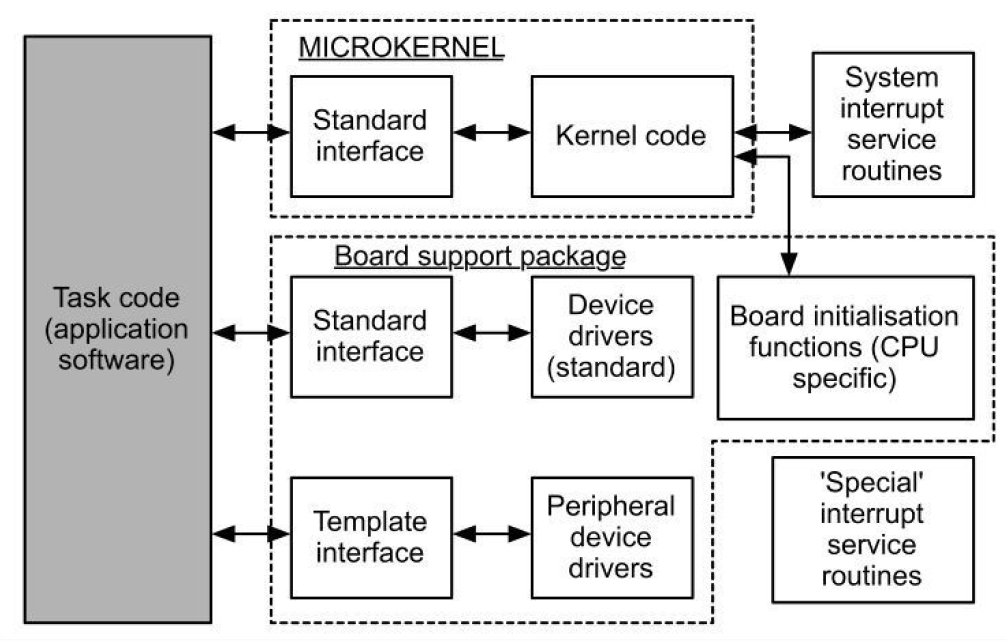
\includegraphics[scale=0.9]{Chapter10/Microkernel.PNG}
        \caption{Software conceptual model - small microkernel-based system}
        \label{fig:microkernel}
    \end{figure}

    \vspace{5pt} \hrule
    
    \item \textbf{Explain what a BSP is and what services it does.} 
    
    BSP = \textbf{B}oard \textbf{S}upport \textbf{P}ackage. The BSP is provided as part of the microkernel package to support both custom and standard hardware designs. Its purpose is to minimize the efforts involved in developing interfacing software for new designs. The BSP offers the following facilities which can be found in many packages:
    \begin{itemize}
        \item Board-specific functions, including general initialization, RTOS initialization and interrupt configuration.
        \item Device-specific driver software, supplied in template form. This is board independent and therefore needs configuration by the programmer.
        \item Detailed low-level code used by the device drivers, but applicable to specific devices (e.g. Intel 82527 communications controller).
        \item Support for the development of special-purpose BSP functions.
    \end{itemize}


    \vspace{5pt} \hrule
    
\end{enumerate}

\end{document}
